
\documentclass[a4paper]{article}
\usepackage{graphicx}
\usepackage{onecolceurwsprofs}
\usepackage{amsmath}
% Dont use mathptmx because mathcal Q for query looks like a mathcal D in times font.
% I.e. mathptmx font is confusing.
% \usepackage{mathptmx}      % use Times fonts if available on your TeX system
% \journalname{Information Retrieval Journal}
%%%%%%%%%%%%%%%%%%%%%%%%%%%%%%%%%%%%%%%%%%%%
%%%%%%%%%% PAPER SPECIFIC STUFF %%%%%%%%%%%%
%%%%%%%%%%%%%%%%%%%%%%%%%%%%%%%%%%%%%%%%%%%%
\usepackage{latexsym}
\usepackage{adjustbox}
\usepackage{paralist}
\usepackage[hang,flushmargin]{footmisc}
\usepackage{url}
\usepackage{tikz}
\usepackage{relsize}
\usetikzlibrary{bayesnet}
\usetikzlibrary{arrows.meta}
\tikzset{vertex/.style={circle,draw,minimum size=1.5em},edge/.style={->,> = latex'}}
\setlength{\textfloatsep}{5pt}
%% \usepackage[font=small,skip=4pt]{caption}
\usepackage{subcaption}
\usepackage{amssymb}
%\usepackage[]{amsthm}
\usepackage[]{mathtools}
\usepackage[]{url,xspace,booktabs,enumitem}
\newcommand{\union}{\cup}
% --------- refcmd ------------ %
\newcommand{\figref}[1]{Figure~\ref{#1}}
\newcommand{\tabref}[1]{Table~\ref{#1}}
\newcommand{\thref}[1]{Theorem~\ref{#1}}
\newcommand{\lemref}[1]{Lemma~\ref{#1}}
\newcommand{\secref}[1]{\S~\ref{#1}}
\newcommand{\ssecref}[1]{Subsection~\ref{#1}}
\newcommand{\charef}[1]{Chapter~\ref{#1}}
\newcommand{\algoref}[1]{Algorithm~\ref{#1}}
\newcommand{\eqnref}[1]{Eq.~\ref{#1}}
\newcommand{\appref}[1]{(Appendix~\ref{#1})}
% ----------- eg ------------ %
\usepackage{xspace}
\newcommand{\eg}{e.g.,\xspace}
\newcommand{\bigeg}{E.g.,\xspace}
\newcommand{\etal}{\textit{et~al.\xspace}}
\newcommand{\etc}{etc.\xspace}
\newcommand{\ie}{i.e.,\xspace}
\newcommand{\bigie}{I.e.,\xspace}
% ---------------- todocmd ----------------- %
\usepackage[color=yellow]{todonotes} % insert [disable] to disable all notes.
\newcommand{\Todo}[2][red]{\todo[]{\textcolor{#1}{\footnotesize #2}}}
\newcommand{\TODOi}[2][red]{\todo[inline]{\textcolor{#1}{\footnotesize #2}}}
% ---------
\usepackage{setspace}
% ---------------- hyperref ----------------- %
% Fix hyperref problem
% https://tex.stackexchange.com/questions/16268/
% warning-with-footnotes-namehfootnote-xx-has-been-referenced-but-does-not-exi
\RequirePackage{hyperref}
\usepackage{xcolor}		% make links dark blue
\definecolor{darkblue}{rgb}{0, 0, 0.5}
\hypersetup{colorlinks=true,citecolor=darkblue, linkcolor=darkblue, urlcolor=darkblue}
% ------- paper specific cmd ------ %
\newcommand{\citer}[1]{{\color{red}#1}}
\newcommand{\E}{\mathrm{E}}
\newcommand{\I}{\mathbf{I}}
\newcommand{\Sigmai}{\Sigma_{(i)}}
\newcommand{\Sigmat}{\tilde{\Sigma}}
\newcommand{\XmD}{\cX \setminus \cD}
\newcommand{\XmQ}{\cX \setminus \cQ}
\newcommand{\Z}{\mathbf{0}}
\newcommand{\alphat}{\tilde{\alpha}_\cQ}
\newcommand{\ath}[1]{#1^{\textrm{th}}}
\newcommand{\bA}{\mathbf{A}}
\newcommand{\bI}{\mathbb{I}}
\newcommand{\bX}{\mathbf{X}}
\newcommand{\bZ}{\mathbf{0}}
\newcommand{\betat}{\tilde{\beta}_\cQ}
\newcommand{\bfZ}{\mathbf{Z}}
\newcommand{\bxui}{\mathbf{x}^{(i)}}
\newcommand{\bx}{\mathbf{x}}
\newcommand{\bzi}{\mathbf{z}_i}
\newcommand{\bzj}{\mathbf{z}_j}
\newcommand{\bz}{\mathbf{z}}
\newcommand{\cA}{\mathcal{A}}
\newcommand{\cD}{\mathcal{Q}}
\newcommand{\cE}{\mathcal{E}}
\newcommand{\cG}{\mathcal{G}}
\newcommand{\cL}{\mathcal{L}}
\newcommand{\cM}{\mathcal{M}}
\newcommand{\cNc}{\mathcal{N}_c}
\newcommand{\cN}{\mathcal{N}}
\newcommand{\cQ}{\mathcal{Q}}
\newcommand{\cDoc}{\mathcal{D}}
\newcommand{\cVp}{\mathcal{V'}}
\newcommand{\cR}{\mathcal{R}}
\newcommand{\cV}{\mathcal{V}}
\newcommand{\cX}{\mathcal{X}}
\newcommand{\eps}{\epsilon}
\newcommand{\ip}[2]{\langle  #1, #2 \rangle}
\newcommand{\lambdat}{\tilde{\lambda}}
\newcommand{\mui}{\mu_{(i)}}
\newcommand{\mut}{\tilde{\mu}}
\newcommand{\pd}{p_{\mathcal{D}}}
\newcommand{\perm}{\sigma}
\newcommand{\px}{p_x}
%\newcommand{\rA}{\mathrm{A}}
\newcommand{\rA}{\mathrm{A}}
\newcommand{\rD}{\mathrm{Q}}
\newcommand{\rDoc}{\mathrm{D}}
\newcommand{\rVp}{\mathrm{V'}}
\newcommand{\rF}{\mathrm{F}}
\newcommand{\rK}{\mathrm{K}}
\newcommand{\rQ}{\mathrm{Q}}
\newcommand{\rS}{\mathrm{S}}
\newcommand{\rV}{\mathrm{V}}
\newcommand{\rX}{\mathrm{X}}
\newcommand{\relu}[1]{\text{relu}(#1)}
\newcommand{\rhot}{\tilde{\rho}}
\newcommand{\softmax}[1]{\text{softmax}(#1)}
\newcommand{\ta}{\theta}
\newcommand{\tq}{\tilde{q}}
\newcommand{\xbar}{\bar{x}}
\newcommand{\xui}{x^{(i)}}
\DeclareMathOperator{\IDF}{IDF}
\DeclareMathOperator{\score}{{score}}
\newcommand{\avgdl}{\bar{L}}
\newcommand{\fcq}{\bar{f}_\cQ}
\newcommand{\talpha}{\alphat}
\newcommand{\tbeta}{\betat}
\newcommand{\bsthresh}{t}
\DeclareMathOperator{\NN}{NN}
\newcommand{\gennn}{\NN^{(g)}_\theta}
\newcommand{\infnn}{\NN^{(i)}_\phi}
\newcommand{\cfont}[1]{{\tt #1}}
\newcommand{\ffont}[1]{\underline{#1}}
\newcommand{\fracil}[2]{{#1}/{#2}}
\newcommand{\btau}{{\boldsymbol\tau}}
\newcommand{\alphatil}{\tilde{\alpha}}
\newcommand{\betatil}{\tilde{\beta}}
\newcommand{\fb}[1]{\textbf{#1}}
\newcommand{\cS}{\mathcal{S}}
% \newcommand{\sumc}{\sum} % \newcommand{\sumc}{}
\newcommand{\sumc}{\raisebox{-0.7ex}{$\mathlarger{\mathlarger{\mathlarger{\mathlarger{\Sigma}}}}$}}
\newcommand{\wTv}{Word2Vecf\xspace}
\newcommand{\setX}{SetExpan\xspace}
\newcommand{\er}{ESE\xspace}
\newcommand{\erLong}{Entity Set Expansion\xspace}
\newcommand{\nvge}{NVSE\xspace}
\newcommand{\nvgeLong}{Neural Variational Set Expansion\xspace}
\DeclareMathOperator{\MLP}{MLP}
\DeclareMathOperator{\Therefore}{Therefore}
\DeclareMathOperator{\sign}{sgn}
\DeclareMathOperator{\DF}{DF}
\makeatletter
\g@addto@macro\normalsize{%
  \setlength\abovedisplayskip{5pt}
  \setlength\belowdisplayskip{5pt}
  \setlength\abovedisplayshortskip{5pt}
  \setlength\belowdisplayshortskip{5pt}
}
\makeatother
%\usepackage[]{natbib}
\newcommand{\mycite}[1]{\cite{#1}}%{\citep{#1}}
\newcommand{\mynewcite}[1]{\cite{#1}}%{\citet{#1}}
\newcommand{\myciteauthor}[1]{\cite{#1}}%{\citeauthor{#1}}
\title{Neural Variational Entity Set Expansion for Automatically Populated Knowledge Graphs}
%\titlerunning{Neural Variational Entity Set Expansion}        % if too long for running head
\author{Pushpendre Rastogi \and Adam Poliak \and
  Vince Lyzinski \and
  Benjamin Van Durme}
%\authorrunning{Short form of author list} % if too long for running head
\institution{%Push \at
  Johns Hopkins University \\
  \texttt{pushpendre@jhu.edu}   %        %  \\
  %% % \emph{Present address:} of F. Author  %  if needed
  %%          \and
  %%          S. Author \at
  %%             second address
}
\date{Received: date / Accepted: date} % The correct dates will be entered by the editor
\begin{document}
\maketitle
\begin{abstract} % [69 Words]
%Information Retrieval Algorithms to extract information from knowledge graphs (KG) are often built for clean, manually curated KGs and do not explain their reasoning. Intelligence analysts (user) are unable to fully incorporate such algorithms in their workflow as users often work with unclean, automatically generated KGs and require interpretable tools. unusable by intelligence analyst because most algorithms are built for clean, manually curated KGs and do not explain their reasoning.
%  We propose Entity Recommendation (\er) as a user-facing task for
%  technologies targeting the automatic construction of Knowledge
%  Bases. Akin to prior entity-focused retrieval definitions, a query
%  consists of one or more entities, with the intent of retrieving
%  similar entities.  Differing from prior work, we focus neither on
%  manually curated knowledge bases, nor collections of entity-labeled
%  documents such as Wikipedia.  Further, we describe an approach
%  for \er, \nvgeLong, which supports human
%  interpretable query rationales, and outperforms baselines
%  such as Bayesian Sets and BM25.
We propose %a new method called
\nvgeLong %(\nvge)
%for \erLong on a noisy KG and a general
to extract actionable information from a noisy
knowledge graph (KG) and
propose a general approach for increasing the
interpretability of recommendation systems. We
demonstrate the usefulness of %our new method on the
applying a variational autoencoder to the
\erLong task %with 
based on a realistic
automatically generated KG.
%We provide
\end{abstract}
\section{Introduction}

Imagine a physician trying to pin-point a specific diagnosis or a journalist %security analyst
investigating
%attempting to uncover 
abuses of governmental power. % local terrorist network. 
In both scenarios,
%the \textit{searcher/user/domain expert} 
a \textit{domain expert} may try to find answers
based on prior known, relevant entities -- either a list of diagnoses
of with similar symptoms that a patient is experiencing or a list of known conspirators. 
%locally known terrorist sympathizers. 
Instead of manually looking for connections between potential answers and prior knowledge, a \textit{searcher}
would like to rely on an automatic \textit{Recommender} to find the connections and answers for them, i.e. related entities.
%\todo{explain why entities search as opposed to keyword search}
 
In the information retrieval (IR) community, Entity Set Expansion (ESE) is the established task of recommending
entities that are similar to a provided seed of entities.\footnote{We refer to the items in
the seed as entities but they can also be referred to as items or elements}
ESE has been applied in Question Answering~\mycite{wang-EtAl:2008:EMNLP2}, 
Relation Extraction~\mycite{lang-henderson:2013:NAACL-HLT} and Information Extraction~\mycite{hegrishman2015demos} settings. 
The physician and journalist in our example can
not fully take advantage of IR advances in ESE for two main reasons. Recent advances 1) often assume
access to a clean, large Knowledge Graph and 2) are uninterpretable.
 
Many advanced ESE algorithms rely on manually curated, clean Knowledge Graphs (KG),
e.g. DBpedia \mycite{auer2007dbpedia} and Freebase \mycite{bollacker2008freebase}. 
%clean KGs duplicate entities are merged, entities rarely are isolated, and entities with similar names
%are properly disambiguated.
In real-world settings, users rarely have access to clean KGs,
and instead %, users 
may rely on automatically generated KGs. Such KGs are often
\textit{noisy} because they are created from complicated
and error-prone NLP processes -- illustrated in \figref{fig:ff1}. %--
For example, automatic KGs may include duplicate entities, associations (relations) between
entities may be missing, and entities with similar names may be incorrectly disambiguated.
%Faulty coreference or entity linking may fail to merge duplicate entities, may create many isolated entities, and may poorly disambiguate entities with similar names.
These imperfections prevent
machine learning approaches %graph-based approaches %analytics %validated on curated KGs
from performing
well on automatically generated KGs. 
%\mynewcite{pujara2017sparsity} and \mynewcite{rastogi2017vertex} show how 
Furthermore, many ESE algorithms degrade as the sparsity and unreliability of KGs
increases~\mycite{pujara2017sparsity,rastogi2017vertex}.
%
Advanced ESE methods, especially those that rely on neural networks, are
uninterpretable \mycite{mitra2017neural}. If a physician can not explain decisions, patients
may not trust her and if a journalist can not demonstrate how a certain individual is acting unethically or above the law,
a resulting article may lack credibility.
%Uninterpretability is a large issue that is general across other fields
Furthermore, uniterpretability may limit the applications of advancements in IR, and more broadly artificial 
intelligence,
as humans ``won't trust an A.I. unless it can explain
itself.''\footnote{\url{https://nyti.ms/2hR1S15}} 


%%%GOALS:
%Problem:
%Given a query of more than one entity, find the most similar entities in the corpus.
%  this can be viewed as a recommendation problem, word-similarity problem, or set-expansion problem, or ad-hoc IR problem.
%We use a 
%
%Evaluation:
%  Compare against state-of-the-art entity set expansion
%  compare against embeddings method
%  compare against standard IR methods
%Unsupervised
%%%

\begin{figure*}[t]
  \centering
  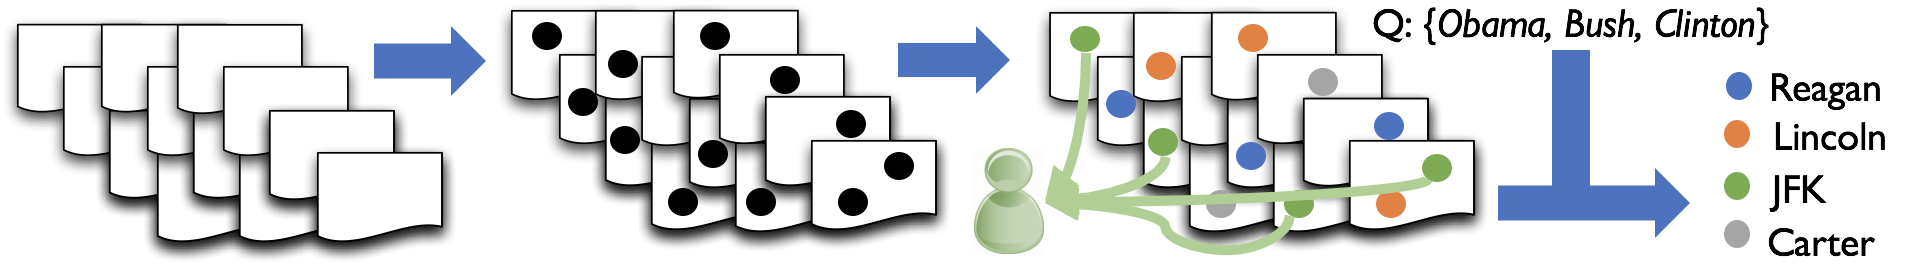
\includegraphics[width=\linewidth,trim=0 0 0 0,clip]{er-pipeline.png}
  \caption{ %\erLong.
    Our \emph{\erLong} (\er) system assumes a corpus that has been labeled with entity mentions which are clustered via cross-document co-reference and linking to a knowledge base; together known as \emph{entity discovery and linking} (EDL). Given a query containing \textit{Obama},
\textit{Bush}, and \textit{Clinton}, the \er system returns other U.S. presidents found in the KG. }
%uses these entities as queries to find other related entities.}% Although we do not explicitly incorporate relationships between entities, our model can be extended to include them.}
  \label{fig:ff1}
\end{figure*}


We introduce \nvgeLong (\nvge) to advance the applicability of ESE research. %address these issues.
 \nvge is an unsupervised model based on Variational Autoencoders (VAEs) that
 receives a query, %consisting of a small set of entities
 uses a Bayesian approach to determine a latent concept
 that unifies entities in the query,
 and returns %both
 a ranked list of %similar entities mentioned in text.
 %relevant information in text
 similar entities based on the previously determined unified latent concept.
 %We refer to our method
 %as \nvgeLong since we 
 %\nvge uses a VAE to %Variational autoencoder to
 %model the latent concept as a Gaussian distributed random variable.
%
 \nvge does not require supervised examples of queries and responses,
 %nor a manually curated KG. It also does not require 
 nor pre-built clusters of entities. % during training. % \Todo{Explain more clearly how the model is estimated. We are not using groups of entities during training. Completely unsupervised training therefore it should be evaluated against other unsupervised methods.}
 Instead, our method
 only requires sentences with linked entity
 mentions, i.e. spans of token associated with a KG entity, %that are
 %always 
 often included in automatically generated KGs.

%We address the first issue %(1)
\nvge %addresses the first issue %because it is more robust than baselines
%by being
is robust to noisy automatically generated KGs, thus removing the need to rely on manually curated, clean KGs.
We evaluate \nvge %outperforming the baselines 
%by evaluating our method 
on the \er %\erLong (\er) 
task using Tinkerbell \mycite{tinkerbell2017Tac},
an automatically generated KG that placed first in the TAC KGP shared
task. 
%\er is the
%task of returning a ranked list of entities %from a KG
%based on a user-specified
%query of entities - \figref{fig:ff1} shows an example of ESE. %for an example of ESE). % where the query contains some U.S. presidents). 
Unlike how ESE has been used to improve entity linking for KG construction~\mycite{gottipati2011linking},
% who use ESE to improve entity linking for KG construction,
our goal is the opposite: %We aim to use noisy KGs for performing ESE.
we leverage noisy automatically generated KGs to perform ESE. % over noisy automatically generated KGs.
%We solve 
\nvge is interpretable; %solves the second issue %(2)
%by outputting 
it outputs \textbf{query rationales} -- a summarization of features
our models associates with the query --
and \textbf{result justifications} -- an ordered list of sentences 
%mentioning the returned entity 
from the underlying corpus
that justify why
our method returned that entity. Query rationales and result justifications are
reminiscent of \textit{annotator rationales}~\mycite{zaidan-eisner-piatko-2008:nips}. %'s \textit{annotator rationales}.


 %Furthermore, t
 To our knowledge this is the first unsupervised
 neural approach for %cold start
 \er as opposed to neural methods for supervised collaborative filtering~\mycite{lee2017augmented}. %, such as \mynewcite{lee2017augmented}.
 All code and data is available at \url{github.com/se4u/nvse} and a video demonstration of the system is available at \url{youtu.be/sGO_wvuPIzM}.

%\section{Entity Recommendation} %Background}

%% In practice, users working with large KGs even now only rely on weighted boolean and keyword searches \mycite{jin2005query,gadepally2016recommender} instead of advanced KG completion algorithms because these tasks: 1) require a \textbf{manually-curated,} and \textbf{clean} KG, 2) do not \textbf{justify} or \textbf{explain} their results; and 3) prevent users from easily \textbf{fine-tuning} their query.

%\noindent
%\par {\bf Existing Issues}
%\subsection*{Motivation}
%The first issue limiting users' ability to incorporate automatically generated KGs with advanced \er
%algorithms %in their workflow
%is that such algorithms %\mycite{zhang2017entity,zheng2017entity} %modern algorithms for \er
%are %either
%validated only on manually curated datasets, e.g. DBpedia and Freebase \mycite{auer2007dbpedia,bollacker2008freebase}.
%In constrast, automatically generated KGs are \textit{noisy} since they contain duplicate entities
%and a large number of entities may be isolated. 
%In contrast, manually curated KGs merge duplicate entities and rarely create isolated entities. 
%
%these algorithms require supervision.
%\mynewcite{manzil2017deep} generate supervised data by clustering words via LDA \mycite{blei2003latent},
%%as a preprocessing step to cluster words in a corpus to generate supervised data %and the clusters as supervised data,
%and
%\mynewcite{vartak2017meta} use manual annotations by twitter users.
%However users typically do not have access to a manually created KG or large amount of annotations; %such annotations or manually created KGs.
%%They
%and instead, work with \textit{noisy} KGs automatically generated from text by NLP systems
%\mycite{rastogi2017vertex}.
%%In brief
%%NLP systems can automatically produce KGs by first performing \textit{named entity recognition} to find mentions of entities,
%%then %\textit{in-document
%\textit{coreference resolution} and \textit{relation extraction} to detect entities' corefernt mentions, properties, and relations
%with one-another,
%coreferent mentions of entities, their properties and relations to other entities,
%and finally \textit{entity linking} to link  coreference chains to a KG.
%Automatically produced KGs are often noisy since there can be many duplicate entities % in an automatically produced KG and
%and a large number of entities may
%not have any connections to other entities.
%be isolated.
%In contrast, manually curated KGs merge duplicate entities and rarely create isolated entities. % isolated from other entities.
% not connected to other entities. % often have many connections.
%These differences
%limit
%prevent graph analytics validated on curated KGs
%from performing %as
%well on automatically generated KGs~\mycite{rastogi2017vertex}.
%\Todo{add note about how we don't use the relations from a KG but we can}


%The second issue preventing users from using advances in NLP is that modern algorithms based on neural networks
%%that outperform traditional keyword information retrieval (IR) systems
%are
%uninterpretable \mycite{mitra2017neural}. This lack of interpretability %is a major hindrance in
%limits
%the adoption of %complicated
%advanced
%methods
%%since
%as users
%%are responsible to
%must justify their actions %or findings
%and humans ``won't trust an A.I. unless it can explain
%itself.''\footnote{\url{https://nyti.ms/2hR1S15}}  %\url{https://www.nytimes.com/2017/11/21/magazine/can-ai-be-taught-to-explain-itself.html}}}
% -- % to people they are advising --
%a physician and a financial adviser must justify their respective medical diagnoses and market
%advice.\footnote{As described in a recent NYTimes article, ``human doctors still have to make the decisions — and they won't
%trust an A.I. unless it can explain itself'' - \url{https://www.nytimes.com/2017/11/21/magazine/can-ai-be-taught-to-explain-itself.html}}
%findings.\footnote{A good physician justifies a choice between diagnoses and a prudent financial adviser
%explains  why she recommended a stock.}
%must be able to
%can
%explains  why she recommended a stock. % over another.}

%The third issue is that
%Additionally, a lack of interpretability
%leads to frustration during production
%because
%when %the
%a
%system does not work as intended -- such as if a recommender system gives inappropriate or inaccurate recommendations --
%it is not possible for an analyst to \textit{patch} the system to correct its output.
%Adding weights to entities in a query allows a user to fine-tune her query.
%In neural \er methods, a user cannot add weights %, either positive or negative,
%to tell a system
%which items in a query to focus more or less on.
%Although well established search methods allow weighted search terms, weights have not been
%incorporated into new methods for \er. %\erLong.
%%nor is it possible for the analyst to know why the system made the wrong recommendation. %in the first place.
%%Because of this
%%In turn,
%%it is not possible to safely
%%and incrementally improve newer systems by making small local changes.
%
%%and interpretable explanations for the rankings.
%%
%%\nvge can be used for many IR tasks of interest
%%to a user %, such as \Todo{list them},
%%%but we focus on
%%We evaluate \nvge on
%%Entity Recommendation (\er), the task of returning a ranked list
%%of entities from a KG that are most related to a query of
%%entities.
%%, and compare it to two strong baselines.
%\noindent
%{\bf Our Contribution}
%\subsection*{Our Contribution}
%Finally, we resolve issue (3) by
%fully incorporating positive and negative feature weights in \nvge. %our \er
%method.
%We introduce a method to provide interpretable explanations for ranking
%and apply this method to \nvge and the baseline models we implement.

\section{Related Work}
%Related work can be grouped into the following clusters:
%stress the 3 issues, super high level overview of the different approaches
%\par{Systems developed on unrealistic data}
%We group related work based on the following categories:
%
%% \noindent
%% {\bf Methods dependent on manually curated KGs.}
%% %\subsection{Methods dependent on manually curated KGs.}
%% Some approaches for ESE only evaluate their methods
%% on manually curated KGs \mycite{zhang2017entity,}.\footnote{
%% Such KGs include DBpedia \mycite{auer2007dbpedia}, Freebase \mycite{bollacker2008freebase}, and Yago \mycite{suchanek2007yago}.}
%% %For example
%% %\mynewcite{zhang2017entity} uses DBPedia \mycite{auer2007dbpedia} and \mynewcite{zheng2017entity} uses Freebase \mycite{bollacker2008freebase}.
%% %e.g. 
%% These improvements
%% %can not be used
%% are not useful for users who deal with noisy, unclean
%% automatically generated KGs.
%% As demonstrated by our experiments, \nvge %Our method
%% is more robust to noisy automatically generated KGs. % and we evaluate it on such a dataset.
\noindent
{\bf Methods dependent on external information.}
%\subsection{Methods dependent on external information.}
%% \Todo{That can be merged with entity set expansion, the next block, at least
%%   the Pasca and Van Durme parts.  See this as another reference to add
%%   lightly, and the text of their Sec 2.4: Web-Scale Distributional
%%   Similarity and Entity Set Expansion}
Since automatically generated KGs can be noisy, 
some methods utilize information beyond entity links and mentions to aid ESE.
\mynewcite{pasca2007you} use search engine query logs to extract attributes related to
entities and \mynewcite{pacsca2008weakly} extract sets of instances associated with class
labels based on web documents and queries.
\mynewcite{pantel-EtAl:2009:EMNLP} use a large amount of web data
as they apply a learned word similarity matrix extracted from
a 200 billion word Internet crawl to the \er task.
Both \mynewcite{he2011seisa}'s SEISA system and \mynewcite{tong2008system}'s Google Sets
use lists of items from the Internet and try to
determine which elements in the lists are most relevant to a query. % of entities.
\mynewcite{sadamitsu-EtAl:2011:ACL-HLT2011} rely on given topic information about the queried entities
to train a discriminative system. 
More recent approaches also use external information.
\mynewcite{manzil2017deep} use LDA \mycite{blei2003latent} to create
word clusters for supervision,
%generate supervised data by clustering words via LDA \mycite{blei2003latent},
and \mynewcite{vartak2017meta} use manual annotations by Twitter users.
\mynewcite{zheng2017entity} uses inter-entity links in knowledge graphs which are very sparse in automatically generated KGs~\mycite{pujara2017sparsity,rastogi2017vertex}.
All of these approaches use more information than just entity links and mentions. % their mentions.

\noindent
{\bf Methods for comparing entities.}
%\subsection{ Methods for comparing entities}
 Set Expander for Any Language (SEAL) \mycite{wang2007language-independent} and its variants \mycite{wang2008iterative,wang2009automatic}
%were early approaches that
learn similarities between new words %entities
and example %entities
words using methods like Random Walks
and Random Walks With Restart.
Similar to \mynewcite{lin1998automatic}'s using cosine and Jaccard similarity to find similar words, %compute word similarity,
%\mynewcite{he2011seisa}
SEISA uses these metrics to expand sets.
% Other methods for computing word similarity, e.g. %have also been explored, e.g. %such as
%sum of
%cosine, Jaccard, and Dice similarities \mycite{lin1998automatic}, can also be .he2011seisa
These methods are limited to only extracting %entities
words that coocur. Because
they are applied on web-scale data, SEAL and SEISA assume entities will eventually coocur.
This assumption might not be valid in an underlying corpus used to automatically generate a KG.
%This assumption breaks under data that users are concerned with, e.g. medical, financial, or news reports.
%Like \mynewcite{ghahramani2006bayesian}'s Bayesian Sets,
In contrast to those approaches, \nvge finds similar entities based on a kernel between distributions.

\noindent
{\bf Queries as natural language.}
%In the INEX-XER shared task \mycite{demartini2009overview}, participants were tasked with
%developing methods for. In the shared task, given a topic  a topic contains a natural language question asking for a list of entities.
In the INEX-XER shared task,
queries were represented as natural language questions \mycite{demartini2009overview}.
\mynewcite{metzger2014aspect} %QBEES
and \mynewcite{zhang2017entity} propose methods to extract
related entities in a KG based on a natural language query.
%However, they do not define a query
%to be a list of entities, but instead use natural language text as the query.
%While %their scenarios are
This scenario is
similar to a person interacting with a system like Amazon Alexa. 
%and require advanced NLP techniques for parsing, 
However, our setup
better reflects %the use case of 
users %extracting 
searching for similar entities in a KG as it is more
efficient for users to type entities of interest instead of natural language text.

\noindent
{\bf Neural Collaborative Filtering.}
We are not the first to incorporate neural methods in a recommendation system.
Recently, \mynewcite{He:2017:NCF:3038912.3052569} and \mynewcite{lee2017augmented}
presented deep auto-encoders for collaborative filtering.
Collaborative Filtering assumes a large dataset of previous user interactions with the search engine. For many domains it is not possible to create such a dataset since new data is added everyday and queries change rapidly based on different users and domains. Therefore, we propose the first neural method which does not use supervision for \erLong.
%% \mynewcite{li2017collaborative} use a citation dataset and their recommendations only include
%% %remove
%% %users with less than ten articles. They only gave recommendations for
%% entities that appeared in at least $10$ articles in the corpus.

%\par{Entity Set Expansion}: SIGIR focus on natural language queries. List out the
%different systems (QBEES) that work on QALD and INEX
%Those who take entities as input are BS and SEISA. We implement BS as a baseline.
%\Todo{write why we choose BS}

%\par{Set completion problem}
%Work like Ben's attribute


%collaborative filtering assumes feedback in the form of blank
%but here we don't
%\Todo{
%
%
% \mynewcite{zhang2016joint}
%web data and query logs. It gives a hueristic for
%solving a NP-hard problem.
% Make different modeling assumptions
%\item Bayesian sets is forced to use simple conjugate prior in its generative model which may fail to capture reality
%
%None of the methods address interpretability, both in terms of explaining
%how their system understood the query and why they returned
%certain results.
%
%None of these methods provide query rational or result justifications and support for weighted, negative
%or positive queries.
%}


\section{Notation}
\label{sec:notation}
Let $\cDoc$ be the corpus of documents and $\cV$ be the vocabulary of tokens that appear in $\cDoc$.  We define
a document as a sequence of sentences and we define a sentence as a sequence of tokens.
Let $\cX$ be the set of entities discovered in $\cDoc$ and we refer to its size as $\rX$.
Each entity $x \in \cX$ is linked to the tokens that mention $x$.\footnote{We ignore confidence scores that entity linking systems often assign to a link because confidence scores will prevent us from using a multinomial distribution to model a document as a bag-of-words.} 
Let $\cVp$ be the set of tokens linked to any $x \in \cX$,
and let $\cM_x$ be the multiset of sentences that mention $x$ in the corpus.
%
For example, consider an entity named ``Batman'' and a document containing three sentences
\{\underline{Batman} is good., \underline{He} is smart. Life is good.\}. ``Batman'' is linked to tokens \underline{Batman}
and \underline{He}, %in the first and second sentence respectively,
$\cVp = \{\text{Batman}, \text{He}\}$, and $\cM_{\text{Batman}} = $  \{\underline{Batman} is good., \underline{He} is smart.\}.


In \er, %the \erLong task,
a system receives %the
query $\cQ$ --
a subset of $\cX$ -- and has to sort the elements remaining in $\cR = \XmQ$.
The elements that are most similar to %the members of
$\cQ$ should appear higher in the sorted order and elements dissimilar to $\cQ$ should be ranked lower.

\section{Baseline Methods}
Before introducing \nvge, we describe the four baselines systems: BM25, Bayesian Sets, \wTv and \setX. We do not compare to DeepSets~\mycite{manzil2017deep}, as it is a supervised method that requires entity clusters.

For each $x$, we create a feature vector $f_x \in \mathbb{Z}^{\rF}$ from $\cM_x$,
by concatenating three  vectors that count how many times
1) a token in $\rV$ appeared in $\cM_x$ 2) a document in $\cDoc$ mentioned $x$ and 3) a token in $\cVp$ appeared in $\cM_x$.
Thus, $\rF = \rV + \rDoc + \rVp$.
% We use the same feature vectors for BM25, BS and \nvge.

%\noindent{\bf BM25}
\subsection{BM25}
%Across all methods, we use the same feature vectors.

Best Match 25 (BM25) is ``one of the most successful text-retrieval algorithms''
\mycite{robertson2009prf}.
%and
%even the apache library Lucence replaced tf-idf with BM25 as its default algorithm.
\footnote{Lucene replaced tf-idf with BM25 as its default algorithm: \url{https://issues.apache.org/jira/browse/LUCENE-6789}}
BM25 ranks remaining entities in $\cR$ according to the score function
%\vspace{-8pt}
\begin{equation*}
\underset{BM}\score(\cQ, x) = {\sum_{i=1}^\rF} {\frac{\IDF[i] f_x[i] \fcq[i] (k_1 + 1)  }{f_x[i] {+} k_{1} (1{-}b {+} b \fracil{\sum_{j} f_x[j]}{\avgdl})}},
%.
\end{equation*}
where
$f_{x}[j]$ denotes the $j$-th feature value in $f_{x}$, $\fcq$ is the sum of $f_x \forall x \in \cQ$ and $\bI$ is the indicator function.
$k_1$ and $b$ are hyperparameters that commonly set to $1.5$ and $0.75$ \mycite{introductionir}. 
$\avgdl$ %above
is the average total count of a feature in the entire corpus %, i.e.
and $\IDF[i]$ is the inverse document frequency of the $\ath{i}$ feature \appref{bm25-idf}.
%have values $1.5$ and $0.75$
% computed as %, where
%$\avgdl = \fracil{\sum_{x \in \cX} \sum_j f_x[j] }{\rX}$,
%$\DF[i] = \sum_{x \in \cX} \bI[f_x[i] > 0]$
%\[
%\vspace{-7pt}
%\begin{align*}
%\IDF[i]= &\log \frac{\rX - \DF[i] + 0.5}{\DF[i] + 0.5} \\
%\DF[i] = &\sumc_{x \in \cX} \bI[f_x[i] > 0].
%\end{align*}
%\]
%We %first compute a feature vector $\fcq$\footnote{The same feature vector is used for all $3$ methods.} for the query $\cQ$
%We %then
%use Gensim~\mycite{rehurek_lrec}'s BM25 implementation %in Gensim~\mycite{rehurek_lrec}
%to
%rank entities in a descending order
%according to the score function

%\vspace{-5pt}
\subsection{Bayesian Sets}
%\noindent
%{\bf Bayesian Sets}
\mynewcite{ghahramani2006bayesian} introduced the Bayesian Sets (BS) method which converts ESE into a bayesian model selection problem.
BS compares the probabilities that the query entities are generated from a single sample of a latent variable $z \in \Delta^{\rF}$ with the probability that the entities were generated from independent samples. $\Delta^{\rF}$ is the $\rF-1$ dimensional probability simplex. Note that $z$ has the same dimensionality as the observed features. Given $\cQ$ and $\pi$, the prior distribution of $z$, BS infers the posterior distribution of $z$, $p(z | \cQ)$, and %then
computes the following score %for each $\forall x \in \cR$:
%%\vspace{-15pt}
\begin{equation}
 \underset{BS}\score(\cQ, x) = %\log \frac{p(x|\cD)}{p(x)} =
 \log \frac{E_{p(z | \cQ)}[p(x|z)]}{E_{\pi(z)}[p(x|z)]}.
\label{eq:bs}
\end{equation}
%%\vspace{-3pt}
\myciteauthor{ghahramani2006bayesian} computed $\score_{BS}$ in close form by
selecting the conditional probability, $p(x|z)$, from an
exponential family distribution and setting $\pi$ to be its conjugate prior.
They showed that if $p(x|z)$ is multivariate Bernoulli then BS
requires a single matrix multiplication \appref{sec:bs}
and we use this setting for our experiments.% \footnote{We also implement Poisson-Gamma and Gaussian-Wishart variants of BS but they did not perform better.}
% They binarize the count vectors $f_{x}$ as described in ~\appref{app:bs-binarize}

\subsection{\wTv}
\mynewcite{levy2014dependency} generalize \mynewcite{mikolov2013distributed}'s Skip-Gram model
as \wTv
to include arbitrary contexts.
We embed entities with \wTv by using the entity IDs as words
\footnote{Converting entity mentions to entity IDs allows us to overcome issues
related to embedding multi-word expressions as explained in \mynewcite{poliak-EtAl:2017:EACLshort}.}
and the tokens in the sentences mentioning those entities as contexts. Note that all tokens in the sentence, except for some stop words, are used as contexts and not just co-occurrent entities.  
We rank the entities in the order of their total distance to the entities in the query set as
\begin{equation}\label{eq:wtv}
  \underset{W2V}\score(\cQ, x) = - \sum_{\tilde{x} \in \cQ} (v_x - v_{\tilde{x}})^2.
\end{equation}
Here, $v_{x}$ represents the L2-normalized embedding for $x$.


\subsection{SetExpan}
\mynewcite{shen2017setexpan} introduce \setX, a SOTA framework combining context feature selection with %a
ranking ensembles, for set expansion. \setX outperformed other SE methods such as SEISA in their evaluation. \setX represents entities by the contexts
that they are mentioned in. For example, the context features for \underline{Batman} from \secref{sec:notation} will be \{\_\_ is good, \_\_ is smart\}. The contexts are used to create a large feature vector which can be used to compute the inter-entity similarity. The authors argue that using all possible features for computing entity similarity can lead to overfitting and semantic drift. To combat these problems \setX builds the entity set iteratively by cycling between a context feature selection step and an entity selection step. In context feature selection, each context feature is assigned a score based on the set of currently expanded entities. Based on these scores, the context-features are reranked and the top few context features are selected. The entity selection proceeds by bootstrap sampling of the chosen context features and using those features to create multiple different ranked lists of entities. Multiple different ranked lists are finally combined via a heuristic method for ensembling different ranked lists to create a new set of expanded entities. This process is repeated to convergence to get the final list of expanded entities.

\section{\nvgeLong} %\nvgeLong}
Like BS, \nvgeLong first determines the underlying concept, or topic, underlying the query
and then ranks entities based on that concept. % (\secref{sec:using-pzcd-to-rank}).
Our method differs from BS
because we  use a deep generative model with a low dimensional concept representation, to simulate how a concept may generate a query. Also we use a ``distance'' (\S~\ref{sec:using-pzcd-to-rank}) between posterior distributions for ranking entities in lieu of bayesian model comparison.
%% This same %% intuition has been implemented in different ways in~\myciter{SEISA, SEAL, QBEES} methods.
%\begin{figure}[t]%[thbp]
%  \centering%  trim={<left> <lower> <right> <upper>}
%  \includegraphics[width=\linewidth,trim=0 0 0 0,clip]{fig/q2.pdf}
%  \caption{The generative model of query generation is shown on the left.
%    The small nodes denote probability distributions.
%    The variational inference model is shown on the right.
%    The transformation from $z$ to $g$ is done via the G-NN
%    and the transformation from $f_x$ to $q_\phi(z|x)$ is done via the I-NN.}
%  \label{fig:q}
%\end{figure}




\subsection{Inference Step 1: Concept Discovery}
\label{sec:latent-concept}
Our model (Fig.~\ref{fig:q}) is as follows: $z \in \mathbb{R}^d$ is a low dimensional latent gaussian random variable representing the concept of a query. $z$ is sampled from a fixed prior distribution $\pi = \cN(\Z, \sigma^2\I)$, i.e. $z \sim \pi$. The members of $\cQ$ are sampled conditionally independently given $z$. $z$ is mapped via a multi layer perceptron (MLP), called $\gennn$, to $g$, the p.m.f.  of a multinomial distribution that generates $f_x$, the features of $x$. $\gennn$ is a neural network with a softmax output layer and parameters $\theta$. $f_x \in \mathbb{Z}^\rF$ are sampled i.i.d. from
$p(f|z,\theta) = \gennn(z)$.\footnote{Our generative model is inspired by \mynewcite{miao2016neural}'s NVDM. %model
They assume that a single latent variable generates only one observation, %;
but we posit that the same
latent variable $z$ generates all %the
observations in $\cQ$.}

In other words, the vector $f_x$ contains the counts of observed features for $x$ that were sampled from $g$, and $g$ was itself sampled by passing a gaussian random variable through a neural network.

\begin{figure}[t]
    \begin{subfigure}[t]{0.4\linewidth}
      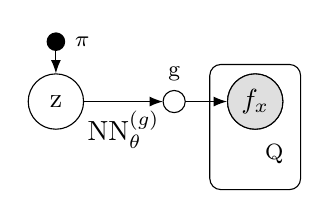
\begin{tikzpicture}%, every node/.style={scale=0.9}
        \node[latent] (alpha) {$\alpha$};%
        \node[obs] (f) {$f_{x}$};%
        \node[latent, left=15pt of f, scale=.4, label=above:g] (g) {};%
        \node[latent, left=of g] (z) {z};%
        \node[fill,circle, scale=.4, above=8pt of z,label=right:$\pi$] (pi) {$\pi$};%
        \plate[inner sep=6pt, yshift=-3pt] {plate1} {(f)} {$\rQ$};%
        \draw[-Latex] (z) -- (g) node[midway, below] {$\gennn$}; %
        \draw[-Latex] (pi) -- (z); %
        \draw[-Latex] (g) -- (f); %
      \end{tikzpicture}
      \caption{Generative Network}
    \end{subfigure}\hspace{0.1\linewidth}
    \begin{subfigure}[t]{0.49\linewidth}
      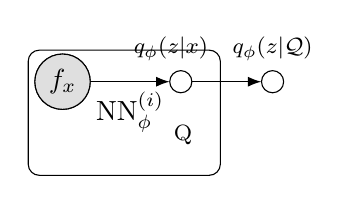
\begin{tikzpicture}
        \node[latent] (alpha) {$\alpha$} ; %
        \node[obs] (f) {$f_{x}$} ; %
        \node[latent, right=of f, scale=.4, label=above:$q_\phi(z|x)\;\;\;$] (zx) {} ; %
        \node[latent, right=25pt of zx, scale=.4, label=above:{$q_\phi(z | \cQ)$}] (zq) {};
        \plate[inner sep=6pt, xshift=4pt, yshift=-5pt] {plate1} {(f) (zx)} {$\rQ$}; %
        \draw[-Latex] (f) -- (zx) node[midway, below] {$\infnn$} ; %
        \draw[-Latex] (zx) -- (zq); %
      \end{tikzpicture}
      \caption{Inference Network}
    \end{subfigure}
    \caption{The generative model of query generation is on the left
      and the variational inference network is on the right.
    Small nodes denote probability distributions,
    gray nodes are observations and the black node $\pi$ is the known prior.
    $\gennn$ transforms $z$ to $g$
    and the $\infnn$ transforms $f_x$ to $q_\phi(z|x)$.}
  \label{fig:q}
\end{figure}

Under this deep-generative model a concept vector can simultaneously trigger multiple observed features. This allows us to capture the correlations amongst features
%that are
triggered by a concept. For example, the concept of \cfont{president}
can simultaneously trigger features such as \ffont{white house}, \ffont{executive order}, or \ffont{airforce one}.

In order to infer the latent variable $z$ ideally we should compute $p_\theta(z|\cQ)$, the posterior distribution of $z$ given the observations $\cQ$. Unfortunately, this computation is intractable because the prior is not conjugate to the likelihood that has a neural network. Another problem is that it is unrealistic to assume access to a large set of ESE queries at training time, because user's information needs keep changing, therefore the approach used by \myciteauthor{manzil2017deep} in DeepSets to discriminatively learn a neural scoring function is \textit{impractical} for set expansion. For the same reason it is also not possible to learn a single neural network whose input is $\cQ$ and which directly approximates $p_\theta(z|\cQ)$. Therefore it is non-trivial to apply the VAE framework to ESE. To overcomes these problems we make the assumption that a query $\cQ$ is conjunctive in nature, i.e. if entity $x_1$ and $x_2$ are present in $\cQ$ then results that are relevant to \textit{both} $x_1$ and $x_2$ simultaneously should be given a higher ranking than results that are related to $x_1$ but not $x_2$ or vice-versa. We implement the conjunction of entities in a query by combining the
\textit{Product of Experts}~\mycite{hinton1999products} approach with the \textit{Variational Autoencoder} (VAE)~\mycite{kingma2013auto} method to approximate $p_\theta(z|\cQ)$.

We first map each $x$ to an approximate posterior $q_\phi(z|x)$ via a neural network $\infnn$ and then we take their product to approximate $p_\theta(z|\cQ)$.
\[
 p_{\theta}(z | \cQ) \approx q_\phi(z | \cQ) \propto \prod_{x \in \cQ} q_\phi(z | x).
\]
The $\phi$ parameters are estimated by minimizing $KL(q(z|x)\mid\mid p(z|x))$ as shown in \S~\ref{sec:est}.\footnote{ %.
%Thus,\footnote{
  This is a generalization of~\mynewcite{bouchacourt2017multi}
  combining variational approximations of posterior distributions
  since the product of gaussians is a Gaussian distribution.}
The benefit of the POE approximation is that the posterior approximation $q_\phi(.|x)$ for each entity $x$ in $\cQ$ acts as an expert and the product of these experts will assign a high value to only that region where all the posteriors assign a high value. Therefore the POE approximation is a way of implementing conjunctive semantics for a query.
Another benefit is that if $q_\phi(.|x)$ is an
exponential family distribution with a constant base measure whose natural parameters are the output of $\infnn$, then the product of the distributions $\prod_x q_\phi(\cdot |x)$ lies in the same exponential family whose natural parameters are simply the sum of individual neural network outputs.\footnote{Also notice that the POE approach recommends adding the \textit{outputs} of the neural networks which is different than concatenating the features for all $x$ in $\cQ$ or naively adding the \textit{inputs} of the neural network. \appref{sec:comp-prod-experts} gives more details.}\textsuperscript{,}\footnote{Recently, \myciteauthor{manzil2017deep} gave a theorem that any permutation invariant function of sets must be representable as the function of a sum of features of elements of the set. We note that our POE approximation also has a similar form and is permutation invariant.}
We use $\infnn$ to compute the mean and log-variance of the gaussian distribution $q_\phi(z  | x)$ (\ref{eq:mean_log-var}) that we
convert to the natural parameters of a Gaussian  (\ref{eq:nat_params_gaus}). %:
Next, we add the natural parameters of the individual variational approximations $\xi_x, \Gamma_x$ to
compute the parameters $\xi_\cQ, \Gamma_\cQ$ for $q_\phi(z | \cQ)$
(\ref{eq:gamma}). % as %such that
Finally, we compute $q_\phi(z|\cQ)$ (\ref{eq:q_phi_z_Q}).
\begin{align}
  \mu_x, \Sigma_x &= \infnn(f_x)\label{eq:mean_log-var} \\
  \xi_x,\ \  \Gamma_x &= \mu_x  \Sigma_x^{-1},\ \  \Sigma_x^{-1}.\label{eq:nat_params_gaus} \\
  \xi_\cQ,\ \ \Gamma_\cQ &= \sumc_{x \in \cQ} \xi_x,\ \ \sumc_{x \in \cQ} \Gamma_x. \label{eq:gamma} \\
  {q_\phi(z|\cQ)} &= \cNc(z | \xi_\cQ, \Gamma_\cQ) \label{eq:q_phi_z_Q}
\end{align}
%As explained above, %the beauty of using the natural parameterization is that
%Now,
%we %can simply
%add the natural parameters of the individual variational approximations $\xi_x, \Gamma_x$ to
%compute the parameters $\xi_\cQ, \Gamma_\cQ$ for $q_\phi(z | \cQ)$ as %such that
%\footnote{$\displaystyle$}.
%\begin{equation}
%  \xi_\cQ, \Gamma_\cQ = \sum_{x \in \cQ} \xi_x, \sum_{x \in \cQ} \Gamma_x. %\\
%  \label{eq:gamma}
%\end{equation}
%Finally, we compute $q_\phi(z|\cQ)$ such that
%\[
%  {q_\phi(z|\cQ)} = \cNc(z | \xi_\cQ, \Gamma_\cQ),
%\]
%where $\cNc(z | \xi, \Gamma)$, the reparameterization of a multi-variate Gaussian distribution, is
$\cNc(z | \xi, \Gamma)$ is the multi-variate Gaussian distribution in terms of its natural parameters --
\[
\frac{|\Gamma|^{1/2}}{(2\pi)^{D/2}}\exp\left(-\frac{(z^T \Gamma z - 2\xi^T z + \xi^T\Gamma^{-1}\xi)}{2} \right).
\]

%% The MLP, $\infnn(x)$, is used to infer the canonical parameters of a gaussian posterior distribution over $z$ given $x$ to match the prior distribution.

%  and the concepts evoked by a document.


%% implement this idea.
%% formalize the intuition that the entities in $\cQ$ where generated from a common concept.

%% Given a query $\cQ$, first we compute the posterior distrubtion over the latent concept $z$.

%% Second we compute the posterior distribution over latent concepts induced by $r \in \cR$. Our score for $r$ is given as

%% Figure~\ref{fig:model} shows our generative model of the queries.

%% We posit that the entities in $\cQ$ were generated from it. A  neural network  maps this low dimensional latent variable to the probabilities of
%% observed features.
% variational auto-encoder to determine the underlying mixture of concepts tying together the queried entities.

% we compute the distribution's distance from the latent content distribution to each remaining entity
%$r \in \cR$ where $\cR = \cX \setminus \cQ$. The distance between the queried entity and a candidate
%entity is defined as

%Going from a low dimensional space to a higher one allows us to model the correlations.
%Consider the following query example \{Obama, Clinton\}
%  provide a lot of power, the probability of different features

%\noindent
%{\bf Step 2: Ranking the remaining entities}
\subsection{Inference Step 2: Entity Ranking}
%\subsection{Metric for entity rankings}
\label{sec:using-pzcd-to-rank}
In order to rank the entities $x \in \cR$, we design a similarity score between
the probability distributions $q_\phi(z|\cQ)$ and $q_\phi(z|x)$ as an efficient substitute for bayesian model comparison.
We use the distance between precision weighted means $\xi_{\cQ}$ and $\xi_{x}$ to define our ``distance'' function as
\begin{equation}
\underset{\nvge}\score(\cQ, x) = -||\xi_{\cQ} - \xi_{x}||^2 .
\label{eq:score_nver}
\end{equation}
Our inter-distribution ``distance'' is not a proper distance because it changes as the location of both the input distributions is shifted by the same amount. We experimented with more standard, reparameterization invariant, divergences and kernels such as the KL-divergence and the Probability Product Kernel \mycite{jebara2004probability}, see \appref{app:rankings}, but we found our approach to be faster and more accurate. We believe this is because the regularization from the prior that encourages the posteriors to be close to the origin makes shift invariance unnecessary.

%Our simple approach
%probability distributions
%\begin{equation}
%\forall x {\in} \cR\,\ d(x, \cQ) = - \ip{ q_\phi(z|\cQ)}{q_\phi(z|x)}  \rangle \label{eq:distance}
%\end{equation}
%which tells us the similarity between the concepts evoked by an entity and the concepts evoked by a query. %% We can compare an entity with a query of entities by comparing $\px = p(z|x)$ and $\pd = p(z|\cD)$.
%If $q(z | \cQ)$ and $q(z | x)$ are very similar that means $x$ and $\cQ$ induce similar distributions over the latent topics and therefore
%$x$ should be ranked higher. In this interpretation, the posterior distribution over the latent variables $z$ induced by $\cQ$ is treated as a semantic hash of $\cQ$ and the
%entire procedure can be considered as a principled way of creating gaussian document embeddings with a generative model instead of using of the ad-hoc approach in~\mycite{vilnis2015word}.
%A standard function for computing the distance between distributions is the KL-divergence.
%Another possibility to compute the distance between distributions is to compute the symmetric version of the KL-divergence.
%Another standard method for computing the similarity between two probability distributions is to compute the probability product kernel between two distributions~\mycite{jebara2004probability}; i.e.
%\[\ip{ q_\phi(z|\cQ)}{q_\phi(z|x)} = \int_z q_\phi(z|\cQ)q_\phi(z|x) dz\]
%In the special case that $q_\phi(z|\cQ)$ and $q_\phi(z|x)$ have the special deep-gaussian form then the KL divergence as well as the inner product can be computed in closed form.
%\footnote{
%  KL Divergence = $\frac{1}{2}(\text{tr}(\Sigma_i^{-1}\Sigma_j) + (\mu_i - \mu_j)^\top \Sigma_i^{-1}(\mu_i - \mu_j) -d - \log \frac{\det(\Sigma_j)}{\det(\Sigma_i)})$.
%
%PPK = $\exp(\frac{-(\mu_1 - \mu_2)^T (\Sigma_1 + \Sigma_2)^{-1} (\mu_1 - \mu_2)}{2} - \log\det((\Sigma_1 + \Sigma_2)))$
%}
%
%However, we propose here an intuitive and simple way to compute the distance between two normal distributions. If $\mu_1, \Sigma_1$ and $\mu_2, \Sigma_2$ are the mean and variance of two normal
%distributions, $p_1, p_2$ then we use the following distance
%\[d(p_1, p_2)  = ||{\mu_1 \Sigma_1^{-1} - \mu_2 \Sigma_2^{-1}}||^2 = ||\xi_1 - \xi_2||^2
%\]
%
%Intuitively this distance gives higher weightage to those dimensions where the variance of the either the distributions is lower. In preliminary experiments we  found this distance to be superior to KL divergence and PPL and we use this distance function in our experiments.
%
%If we use the natural parameterization to represent a Multivariate Normal distribution to represent $q_\phi(z | \cQ)$ and $q_\phi(z|x)$ such that:
%\begin{align}
%  {q_\phi(z|\cQ)} &= \cNc(z | \xi_\cQ, \Gamma_\cQ)\\
%  {q_\phi(z|x)} &= \cNc(z | \xi_x, \Gamma_x)
%\end{align}
%then we can use $\xi$ itself as a point representation of the gaussian distribution and let
%$\displaystyle
%d(x, \cQ) = || \xi_\cQ - \xi_x ||^2
%$
%% Intuitively this distance gives higher weightage to those dimensions where the variance of the either the distributions is lower. In preliminary experiments we  found this distance to be superior to KL divergence and PPL and we use this distance function in our experiments.
%% If we use the natural parameterization to represent a Multivariate Normal distribution
%% to represent $q_\phi(z | \cQ)$ and $q_\phi(z|x)$ such that:
%% \begin{align}
%%   {q_\phi(z|\cQ)} &= \cNc(z | \xi_\cQ, \Gamma_\cQ)\\
%%   {q_\phi(z|x)} &= \cNc(z | \xi_x, \Gamma_x)
%% \end{align}
%% then we can use $\xi$ itself as a point representation of the gaussian distribution and let
%% $\displaystyle
%% d(x, \cQ) = || \xi_\cQ - \xi_x ||^2
%% $

%\noindent
%{\bf Estimating $\theta$ and $\phi$} %under the VAE Framework}
\subsection{Unsupervised Training}
%\subsubsection{Estimating $\theta$ and $\phi$} %under the VAE Framework}
\label{sec:est}
%% VAEs are a combination of deep neural generative models and deep approximations of posterior distributions of such generative models.
%% Modeling
\nvge is trained in an unsupervised fashion to learn its parameters $\theta$ and $\phi$.
\mynewcite{kingma2013auto,rezende2014stochastic} proposed the VAE framework for
learning richly parameterized conditional distributions $p_\ta(x | z)$ from unlabeled data.
We follow \myciteauthor{kingma2013auto}'s reparameterization trick to train a VAE and maximize
the \textit{Evidence Lower Bound}:
\begin{align}
  E_{q_\phi(z | x)}[\log p_\theta(x | z)] - KL(q_\phi(z|x) || p(z)).\label{bound:vae}
\end{align}
During training, we do not have access to any clustering information or side information that tells us which entities can be grouped together.
Therefore we assume that the entities $x \in \cX$ were generated i.i.d. 
%In other words,
The model during training looks the same as \figref{fig:q} but with one difference: $Q$ is a singleton set of just one
entity.\footnote{More informally, we remove the plates from \figref{fig:q}.} % during training.}
Note that our learning method requires no supervision in contrast to methods like Deep Sets which require cluster information, or Neural Collaborative filtering methods which require a large dataset of user interactions.

%% There are other lower bounds  is an improved bound proposed by \mynewcite{burda2015importance}.
%% \mynewcite{cremer2017reinterpreting} construct
%% a special distribution $\tq$ under which the IWAE bound reduces to the VAE bound. Similarly more complicated posterior distributions based on normalizing flows could be used.
%% By optimizing parameters $\phi, \theta$ together we can maximize the lower bound on
%% the marginal probability of the data.
%To learn the parameters during training, we update $\phi$ and $\theta$ using stochastic back-propagation
%as described in \S 2 from \mynewcite{miao2016neural}.
%% We update $\phi$ and $\theta$ using stochastic back-propagation during training
%% as described in \S 2 from \mynewcite{miao2016neural}
%% \subsection{Extension to VAEs}
%% We now present our extension to the VAE framework. The first technical challenge in
%% NVER is computing $p(z | \cD)$. The original VAE framework assumes that each observation is
%% generated i.i.d. and trains a recognition network $q(z | \xui)$ to approximate
%% the posterior $p(z | \xui)$. Instead we need to compute $q(z | \cQ)$ which is.
%% The second technical challenge is that computing the true marginals $p(x | \cD)$ can be too computationally demanding for large collections so we propose efficient alternatives for computing the Bayesian Sets score.
%% \subsection{Approximating $p(z | \cD)$}
%% \label{sec:approximating}
%% In order to approximate $p(z | \cD)$ we propose to use the approximation $q_\phi(z | \cD) \propto \prod_{i=1}^{\rD} q_\phi(z | \xui)$. For \textit{deep-exponential family distributions} the product of experts can be computed by simply adding the sufficient statistics.

%\subsection{Support for weighted queries} %with negative weights}
%\section{Weighted queries}
%\label{sec:weighted-queries}
%Useful recommendation systems for users should be tunable.  If a
%recommendation system returns undesirable entities in response to the
%query, then %it should be possible for
%the user should be able to easily tune the
%query so that the system excludes the undesirable results.
%%Most search engines allow boolean exclusion operators or weighted query
%%terms, but in the \er systems presented so far, a user can only change a
%%query by either removing or adding entities.
%%Furthermore,
%Weighted-queries enable users to tell the system what aspects of the
%query to focus on or ignore.
%
%%For the weights on the entities to be interpreted as the amount of

%To apply user provided weights as the amount of
%influence that an entity should have on the final posterior over
%topics, we integrate the weights directly into the computation of the
%topic posteriors.  If the user provides weights
%$\btau = \{ \tau_x \mid x \in \cQ\}$, %then
%we compute the query features as %follows:
%%\vspace{-1pt}
%
%\begin{equation}\label{eq:weight}
%\xi_{\cQ,\btau},\ \ \Gamma_{\cQ,\btau} = \sumc_{x \in \cQ} \tau_x \xi_x,\ \ \sumc_{x \in \cQ} |\tau_x|\Gamma_x.
%\end{equation}
%%%\vspace{-1pt}
%BM25 supports weights by multiplying each $f_x$ by $x$'s weights when computing $\fcq$. %in the summation in (\ref{eq:bm25_fbar}).
%It is not clear how to incorporate weights in Bayesian Sets.
%%% instead of computing $\Gamma_\cQ = {\sum_{x \in \cQ}\infnn(x)}$
%%% in (\ref{eq:gamma}),
%%% we perform a weighted sum
%%% \[\Gamma_{(\tau, \cQ)} = {\sum_{x \in \cQ}|\tau_x| \infnn(x)}\]
%%% Note that in computing the precision $\Gamma$  we only use the magnitude of the provided weights.
%%% To allow a user to tell the system to focus specificially on entities \textit{NOT} similar
%% to a specific $x$, we enable a user to add negative weights.
%% \textit{Add example}
%% The signed weights are used for computing $\xi$ as follows:
%% \[
%% \xi_{(\tau, \cQ)} = {\sum_{x \in \cQ} \tau_x \xi_{x}}
%% \]

\section{Interpretability}
\label{sec:query-rational}
%Interpretiability has not been given enough attention in the literature.
We introduce a general approach %for making \er models interpretable
for interpreting \er models
%to users %. We
%based on
%and
%apply it to
%demonstrate how %our this approach %can may be applied to
%NVER and our baselines.
%the models discussed.
%\nvge, BM25, and BS.
%the three models.
%not only our method NVER but also our baselines.
%Since \nvge contains two distinct components described in
%\secref{sec:latent-concept} and \secref{sec:using-pzcd-to-rank},
%we provide a general approach to interpret the two components independently:
%Our method contains two distinct components -- determining the
%latent concept unifying the query \ref{} and scoring each entity
%in an automatically generated KG based on that concept \ref{}.
%To enable users to incorporate our method in their workflow, we provide
%an way to understand how our method is working.
%We propose using
based on \textit{query rationales} to explain the latent concept the model discovered
and \textit{result justifications} to provide evidence %to users
for why the system ranked an entity highly. % was ranked highly.
%
%Useful recommendation systems for users should be tunable.  If a
%recommendation system returns undesirable entities in response to the
%query, then %it should be possible for
%the user should be able to easily tune the
%query so that the system excludes the undesirable results.
%%Most search engines allow boolean exclusion operators or weighted query
%%terms, but in the \er systems presented so far, a user can only change a
%%query by either removing or adding entities.
%%Furthermore,
%A user can take advantage of our approach to make \er models more inter
Based on query rationales and result justifications, users can add weights to entities
in a query %Weighted-queries enable users 
to tell the system what aspects of the
query to focus on or ignore. % We note that there are \todo{What do we note, or should this just be removed
%% We demonstrate how these can be applied to \nvge and some of the baseline models.

\subsection{Query Rationale}
A \textit{Query Rationale} is a visualization of the latent beliefs of the \er system given the query $\cQ$. 
Given $\cQ$, we construct a feature-importance-map $\gamma_{\cQ}$ that measures the relative importance of the features
in $f_x$ and we show the top features according to $\gamma_\cQ$ as ``Query Rationales''. Recall that the $\ath{j}$ component of $f_x$, associated with entity $x$, measures how often the $\ath{j}$ feature co-occurred with $x$. We now present how we construct $\gamma_\cQ$ for 
\nvge and the baselines. %our system and under the baselines.

For BM25, $\gamma_{\cQ}$ is simply $\bar{f_{\cQ}}$. % computed in (\ref{eq:bm25_fbar}).
In BS, $\gamma_{\cQ}$ is the weights from (\ref{eq:bs_score}): %, i.e.
for each  $\ath{j}$ component of $f_x$,
\begin{equation*}
\gamma_{\cQ}[j] = \log \frac{\talpha[j] \beta[j]}{\alpha[j]\tbeta[j]}. %,
\end{equation*}
%i.e. the weights from (\ref{eq:bs_score}).
The benefit of generative methods such as BS and \nvge is that for them query rationales can be
computed as a natural by-product of the
generative process instead of as ad-hoc post-processing steps.
For \nvge, ideally $\gamma_{\cQ}$ should be the posterior distribution $p_\theta(f | \cQ)$.
Since this is intractable we approximate it by sampling the inference network:
\[
p_\theta(f | \cQ) = E_{p_\theta(z | \cQ)} [p_{\theta}(f | z, \cQ)]  \approx E_{q_\phi(z | \cQ)} [p_{\theta}(f|z)] .
\]
We further approximate the expectation with a single sample of the mean of $q_\phi(z | \cQ)$.
Finally the feature importance map for \nvge is:
\[\gamma_{\cQ} = p_\theta(f | E[q_\phi(z | \cQ)]).\]
Because \wTv finds the nearest-neighbor between entity embeddings, which are produced through a complicated learning process operating on the whole text corpus, it does not provide a natural way to determine the importance of a single sentence and therefore it is not possible to say what was the effect of a particular sentence on the query results. Similarly, since the \setX method works by extracting context features and iteratively expanding this feature set, it is not possible to determine the effect of a single sentence on the final search results.
%% \todo{(DONE) add a sentence why we cant for the other two baselines}
\subsection{Result Justifications}
%\noindent
%{\bf Result Justifications}
We define
result justifications as sentences in $\cM_{x}$ that justify why an
entity was ranked highly for a given query.
%Besides for a small pre-processing twist,
Ranking the sentences that mention an entity is similar to %identical as
ranking entities in $\cR$. %based on a query.
%Instead of creating a feature vector for each $x$, we create a feature vector for
Just as we create a feature vector for each $x$,
we create a feature vector for
each sentence in $\cM_{x}$ and use the same scoring function to rank the sentences
based on the query.
While computing a score for entity $x$ based on a query,
we also score each sentence in $\cM_{x}$.
%Thus,
Our approach to generate interpretable result justifications is agnostic to \er methods
with the caveat that for methods like \wTv and \setX this will require retraining or reindexing over the corpus for each query. Our approach will not be feasible for such methods.
%% as we can easily swap scoring methods.
%% %We believe that
%% Result justifications provide evidence %to users
%% explaining %why an entity was ranked highly.
%% an entity's ranking.

\subsection{Weighted queries}
Any recommendation system can occasionally fail to provide good results for a query. To improve a %ESE
system's responses in such cases we enable users to guide \nvge's results 
%recommendations 
by using entity weights to influence the posterior distribution over topics.  

If a user provides weights
$\btau = \{ \tau_x \mid x \in \cQ\}$, we compute the query features as
\begin{equation}\label{eq:weight}
\xi_{\cQ,\btau},\ \ \Gamma_{\cQ,\btau} = \sumc_{x \in \cQ} \tau_x \xi_x,\ \ \sumc_{x \in \cQ} |\tau_x|\Gamma_x.
\end{equation}
The above formulae have an intuitive explanation:
 when an entity has a higher weight then the precision over the concepts activated by that entity is increased according to the magnitude of the weight, and the value of the precision weighted mean is also weighted by the user supplied weights. 
%This has the nice outcome that 
In turn, an entity with zero weight has zero effect on the final search result and entities with a high negative weight return entities diametrically opposite to that entity with higher confidence.

Weights can be applied to other methods as well. 
BM25 %supports weights by multiplying each
can multiply each
$f_x$ by $x$'s weights when computing $\fcq$,
and \wTv can %incorporate weights by using
use a weighted average.
It is not straight-forward to incorporate weights in BS and \setX systems. One possible way is to use bootstrap resampling of the query entities according to a softmax distribution over entity weights, but bootstrapping makes the system non-deterministic and therefore even more opaque for a user. Also bootstrap resampling requires multiple query executions and it is not straight-forward to combine the outputs of different search queries; therefore we do not advocate for bootstrapping. %this method.

%Summarize section 3 in NVDM paper~\mycite{miao2016neural} and add our own figure.
%\Todo{We need to explain the two MLP we use, and the model that generates the natural parameters.}

\section{Comparative Experiments}
%% Our proposed method determines the latent random variable
%% responsible for generating the query and then ranks the entities
%% in $\cR$ by computing a distance between the probability of the
%% latent variable given the given query and the probability of the
%% latent variable given each entity.
We test the hypothesis that \nvge can help bridge the gap between advances in IR and real world use cases. We use human annotators on Amazon Mechanical Turk (AMT) to determine whether \nvge finds more relevant entities than our baseline methods in a real world, automatically generated KG.

% to evaluate whether \nvge converges during training. %the objective function
%2) weights help users fine tune queries;
%2) \nvge's query rationales accurately describe the latent concept unifying our queries;
%3) \nvge's result justifications provide useful descriptions of the ranked entities.
%1) our entity rankings are better than other methods.
%2) our rationales are good; 3) our justifications are good.
%
%\paragraph{Dataset}

%\noindent
%{\bf Dataset}
\subsection{Dataset}
TinkerBell~\mycite{tinkerbell2017Tac} is a KG construction
system  that achieved top performance in TAC-KGP2017
evaluation.\footnote{Tinkerbell constructed a KG from %TAC KGP 2017
\texttt{LDC2017E25} %,  %\footnote{\texttt{LDC2017E25}}
that contains $30K$ English documents.
Half of them are from online forums and
the other half from Reuters and NYT.
We focused on the $77,845$ entities from English documents appearing in $344,735$ sentences.
$25,149$ entities were also linked to DBPedia.}
We used it as our automatic KG. For each entity $e$ in TinkerBell we create $\cM_e$ by %collecting
concatenating all %the
sentences that mention $e$ and  remove the top $100$ most frequent features in the corpus from $\cM_e$ to clean stop words.
Tinkerbell was constructed from the TAC KGP 2017 evaluation source
corpus, \texttt{LDC2017E25}, that contains 30K English documents and 60K Spanish and Chinese documents. \footnote{\url{tac.nist.gov/2017/KGP/data.html}}
Half of the English documents come from online discussion forums and the other half from
news sources, e.g. Reuters or the New York Times.
Our experiments only use the 77,845 EDL entities within TinkerBell that are assigned the type \texttt{Person}. We use these links to create a map from DBPedia categories to entities in TinkerBell, say $M$. Each entity in TinkerBell is associated to spans of characters that mention that entity. We tokenize and sentence segment the documents in LDC2017E25 and associate sentences to each entity corresponding to mentions. In the end we get 344,735 sentences associated to the 77K entities. The median number of sentences associated to an entity is $1$ and the maximum number of sentences is $4638$ for the \textit{Barack Obama} entity.\footnote{The mean is 4.43, %4.284796711413703,
the standard deviation is 29.19, %29.187011229612995,
the minimum number of sentences for an entity is 1,
the maximum number of sentences is 4638,
and the median is 1 (44,317 entities).} This is a good example of how automatic KGs differ from manually curated KGs. In TinkerBell most of the entities appear in only a single sentence so only a single fact may be known about them. In contrast KGs like FreeBase and DBPedia have a more uniform coverage of facts for entities present in them. Another difference is that relational information such as ancestry relations between entities are much more noisy in an automatically generated KB than in DBPedia which relies on manually curated information present in Wikipedia.



\subsection{Implementation Details}
We prune the vocabulary by removing any tokens that occur less than $5$ times across all entities.
%% \footnote{
%% Pruning minimizes training and query time;
%% smaller pruning would make the system to slow during recommendation.}
We end up with, $\rF {=} 105448, \rV = 61311$, $\rDoc =  24661$, and  $\rVp = 19476$.
We used BM25 implemented in Gensim~\mycite{rehurek_lrec} and we
implemented BS ourselves. %For BM25, following common practice, we set $k_1$ as $1.5$ and $b$ as $0.75$, and 
%For BS,
We choose $\lambda=0.5$, out of $0$, $0.5$, or $1$, after visual inspection. We used 
\wTv and \setX codebases released by the authors.\footnote{\url{https://bitbucket.org/yoavgo/word2vecf}, \url{github.com/mickeystroller/SetExpan}}
For \nvge, we set $d{=}50$, $\sigma{=}1$. The generative network $\gennn$ does not have hidden layers and the inference network $\infnn$ has $1$ hidden layer of size $500$ with a $\tanh$ non-linearity and two output layers for the mean $\mu_x$
and log of the diagonal of the variance $\Sigma_x$. We use a diagonal $\Sigma_x$.
\footnote{Training \nvge on $1$ Tesla K80 using the Adam optimizer %% \mycite{kingma2014adam}
  with learning rate $5e^{{-}5}$
  and minibatch size $64$ took $12$ hours.}
For \wTv, we used $d=100$ to use the same number of parameters per entity as in \nvge. We trained with default hyperparameters for 100 iterations. We used \setX with the default hyperparameters as well except that we limited the number of maximum iterations to $3$ since we only needed top $4$ entities for our experiments.
% but query time is roughly $150$ milliseconds.}
%since we export the model from Tensorflow
%after training.
%We use the same features across systems for fair comparison so $F{=}105,448$ for all  systems.


\subsection{Experimental Design}
Prior work typically evaluates ESE on a small number of queries, constituting the most frequent entities, e.g. \myciteauthor{ghahramani2006bayesian} reported results for $10$ queries with highly cited authors and \myciteauthor{shen2017setexpan} used 20 test queries created of 2000 most frequent entities in Wikipedia. However in automatic KGs, most entities are mentioned only a few times. For example 60\% of the entities in TinkerBell are mentioned once. We are primarily interested in unbiased evaluation over such entities, therefore we stratified the evaluation queries into three types.

 The 1st type contains entities mentioned in only $1$ sentence, the 2nd contains entities appearing in $2-10$ sentences, and the 3rd contains entities mentioned in $11-100$ sentences. We also stratified queries based on whether they had $3$, or $5$ entities. 
For each query type we randomly generate 80 queries by first sampling 80 Wikipedia categories and then sampling entities from those categories that were also part of the TinkerBell KG. This %process
results in $480$ queries. See \tabref{tab:qex} for examples.

%% We do not experiment with queries containing $1$ entity since such queries are unsuitable for \nvge's concept discovery. 
%% Randomly selecting entities may result in queries that have no unifying concept. Therefore, we manually remove such queries, resulting
%% in ~XX queries per setting.
%However, due to imperfect entity linking and coreference in an automatically generated KG %%a large number of entities
%many entities may appear in only one sentence while other entities may appear in many more:
%our KG roughly $44K$ of the total $77K$ entities
%appear in only one sentence and only $7$ entities appear in more than $1K$ sentences.\footnote{The mean, std., max and median numbers of sentences that an entity appears in are $4.43$, $29.19$, $4638$ and $1$ respectively.%(44,317 entities).}
%}
%Thus, a purely random method for query selection will cause our experiments to be overly focused on tail queries without enough observations. Therefore We use a stratified procedure to select queries.
%
%We define $12$ types of queries based on $n$ and $s$. $n$ is the number of entities in the query that varies between $1$, $3$ and $5$ and $s$ is the bin based on the size of $\cM_x$ for the entities $x$ in the query. We grouped the entities into binsb ased on whether $|\cM_x| {=} 1,\  2 {\le} |\cM_x| {\le} 10,\  11 {\le} |\cM_x| {\le} 100$ and $|\cM_x| {\ge} 101$.
%For each $s$ we sample $n$ entities as follows: We say that an entity $x$ is eligible if $\cM_x$ lies within $s$. Given $n$ and $s$ we say that a category is eligible if it is mapped to at least $5$ and up to $15$ eligible entities. %% Given $n,s$
%We sample upto a maximum of $80$ categories without replacement from the set of eligible categories. After sampling an eligible category we randomly sample $n$ distinct entities associated to that category. E.g. given a bin $s$ of $1$ sentence and $n=1$ there are a total of $2746$ elgiible categories from which we may sample a category such as \texttt{Indian Film Actors} that contains $15$ eligible entities and we can sample the entity ``John Abraham''.
%This creates $80\times 9 + 27\times 3= 801$ queries. $27$ queries are created when $s=\ \ {>}100$.


%% We create four groups of queries based on the
%% number of sentences that mention a given entity.
%% The first group contains entities that appear in only
%% 1 sentence, the second group contains entities that
%% appear in 2 to 10 sentences, the third group contains
%% entities that appear in 11 to 100 sentence, and the
%% final group contains entities that appeared in $>$100
%% sentences. These groups will allow us to test our
%% our method in a  wide-range of situations.
%% In each group, we determined which concepts
%% in DBpedia linked to between 5 and 15 entities in
%% the given group. Next, for $m \in \{1, 3, 5\}$, we
%% randomly selected $80$ concepts for the first three groups
%% and $27$ concepts for the last group since there only exist $27$ concepts
%% with $5$ to $15$ entities that appear in $>$100 sentences.
%% Finally, we randomly sampled $x$ entities from each %of those
%% concept’s linked entities that appear in the
%% given group. This creates a total of 801 queries: $720$ queries from 3
%% groups, 3 different numbers of entities in a query,
%% and 80 DBpedia concepts; and $81$ queries from 1 group, 3 different number of entities in query, and 27 DBpedia concepts.
%
%\subsection{Experimental Protocol} % and Results} % of Rankings}
%Using all $801$ queries,

%For each query, we showed AMT crowd-source workers a list of the top $4$ entities returned by
%each system. We asked workers to rank \nvge and the baselines based on the lists of
%returned entities.
%We asked workers on AMT to compare \nvge and the baseline systems based on
%the top 4 entities, different from the query entities, returned by them for all $480$ queries\todo{the first sentence is super wordy and a big confusing}.
For each query, we showed the names and first paragraphs from the Wikipedia abstracts of the query's entities, to help the AMT workers disambiguate entities unfamiliar to them. Then we showed the workers the top $4$ entities returned by each system.
Each resultant entity was shown with up to 3 \textit{justification} sentences.\footnote{Figure~\ref{fig:hit_system} in \appref{app:mturk-hit} illustrates the AMT interface.} Since \setX and \wTv do not return justifications, we used \nvge to extract justifications for their results. We asked workers to rank the systems between $1$, the best system, to $3$, the worst; and we allowed for ties. The annotators found it difficult to compare results from 5 systems at a time
so we split our evaluation into two groups. Group 1 compared \nvge to BS and BM25, and group 2
compared \nvge to \setX and \wTv. We randomized the placement of the lists so that the workers could not figure out which system created which list.

\begin{table}[t]
  \centering
  %% \renewcommand{\arraystretch}{1}\linespread{1}\selectfont\centering
  \setlength{\tabcolsep}{4pt}
  \begin{tabular}{| p{3cm} | p{4.5cm} |}\hline
    \textbf{Category} & \textbf{Entities}\\[-1pt]\hline
    (1 Sent./Ent.) Am- erican Jazz Singers   & Paula West, Natalie Cole, Chaka Khan \\\hline
     (2-10 Sent.) Austr- alian Major Golfers & Marc Leishman, David Graham, James Nitties\\\hline
     (11-100 Sent.) The Apprentice (U.S) Contestants& Maria, Rod Blagojevich, Dennis Rodman, Joan Rivers, Piers Morgan\\\hline
  \end{tabular}
  \caption{Examples of randomly created queries}
  \label{tab:qex}
\end{table}

%, as described in \S\ref{sec:query-rational}.
%For each query, we showed the annotators the names of the entities in the query
%and the first paragraph from the entities' Wikipedia pages that we extracted from DBPedia.
%For each entity returned by the systems,
%we also showed workers up to 3 \textit{justification} sentences from the corpus that mentioned the entities.
%The justfication sentences were selected using the method described in \S\ref{sec:query-rational} for selecting result justifications.

%\noindent
%{\bf Results} % and Discussion}
%% \par{Results}
%% %Using \mynewcite{sakaguchi-post-vandurme:2014:W14-33}'s clustering technique for
%% %TrueSkill \mycite{herbrich2007trueskill}, we determine that \nvge, BS, and BM25 overall rank as $1^{st}$, $2^{nd}$, and $3^{rd}$ respectively.
%% %\figref{fig:true_skill} in \appref{app:exp_1} illustrates the results from TrueSkill. % shows each system's rating and seperate clusters based on TrueSkill.
%% For comparing \er systems, we rely on
%% \mynewcite{sakaguchi-post-vandurme:2014:W14-33}'s protocol employed in the 2014-2016
%% %system evaluations of the
%% Conference on Machine Translation (WMT)'s system evaluations %.
%% \mycite{bojar-EtAl:2014:W14-33,bojar-EtAl:2015:WMT,bojar2016findings}.
%% This is based on annotators ranking the %anonymized and randomly ordered
%% output of different systems for each prompt (query), then
%% converting this ordering into a series of pair-wise win-loss-ties,
%% followed by an application of the TrueSkill\texttrademark algorithm
%% \mycite{herbrich2007trueskill} for determining competitor rankings.
%% The protocol ranks \nvge, BS, and BM25 overall as $1^{st}$, $2^{nd}$, and $3^{rd}$ respectively
%% and with a clean break between the systems.
%% ~\tabref{tab:breakdown_rating} records the results broken down
%% by each query setting.



%\begin{table}[htbp]
%  \setlength{\tabcolsep}{3.5pt}
%  \centering
% \begin{tabular}{h|h|hhh}
%\toprule
%Entities   & Sentences  &         & Systems &       \\\cline{3-5}
% Per Query & Per Entity & \nvge   & SetEx   & W2Vec \\\hline
%           & 1          & \fb{51} & 14      & 15    \\
%3          & 2-10       & \fb{49} & 13      & 18    \\
%           & 11-100     & \fb{44} & 10      & 26    \\\hline
%           & 1          & \fb{58} & 19      & 3     \\
%5          & 2-10       & \fb{53} & 19      & 8     \\
%           & 11-100     & \fb{52} & 11      & 17    \\\hline\hline
%           & Total      & \fb{307} & 86      & 87    \\\bottomrule
%\end{tabular}
%  \caption{\nvge versus \wTv and \setX}
%  \label{tab:new-sys}
%\end{table}

\begin{table}[t]%[htbp]
  \setlength{\tabcolsep}{1.75pt}
  \centering
\begin{tabular}{|c@{\hskip 1pt}|r|ccc||ccc|}\hline
  {\small Ents$.$ In}  & {\small Sents. }  &          \multicolumn{3}{c||}{Group 1}      &          \multicolumn{3}{c|}{Group 2}       \\[-2pt]\cline{3-8}
  {\small Query} & {\small Per Ent.} & {\small \nvge}    & {\small BM25}    & {\small BS}  & {\small \nvge}    & {\small SetEx}   & {\small W2Vecf} \\\hline
            & 1          & 27       & \fb{38} & 15  & \fb{51}  & 14      & 15    \\[-1pt]
3           & 2-10       & \fb{29}  & 25      & 26  & \fb{49}  & 13      & 18    \\[-1pt]
            & 11-100     & \fb{35}  & 23      & 22  & \fb{44}  & 10      & 26    \\[-1pt]\hline
            & 1          & \fb{38}  & 25      & 17  & \fb{58}  & 19      & 3     \\[-1pt]
5           & 2-10       & \fb{40}  & 27      & 13  & \fb{53}  & 19      & 8     \\[-1pt]
            & 11-100     & 24       & \fb{33} & 24  & \fb{52}  & 11      & 17    \\[-1pt]\hline\hline
            & Total      & \fb{193} & 171     & 117 & \fb{307} & 86      & 87    \\[0pt]\hline
\end{tabular}
\caption{The number of times a system was ranked $1^{st}$ over 80 queries compared to other systems in the same group. Ties were allowed so some rows may not sum to 80. Bold highlights the system with the most $1^{\text{st}}$ in its group. Extended results with second and third place rankings of the system are shown in \tabref{tab:old-sys-23}.}
\label{tab:old-sys}
\end{table}


\subsection{Results}
\tabref{tab:old-sys} %and \ref{tab:new-sys} 
shows the number of times the
annotators ranked each system as the best out of the $80$ queries. Over all queries, \nvge returned better results compared to the $4$ baselines systems. It performed best with 5 entities in the query where each entity was only mentioned up to $10$ times in the corpus. This shows that \nvge is able to discern better quality topics from multiple entities with sparse data. Extended results showing second and third place rankings of the systems are given in \tabref{tab:old-sys-23} in the appendix which show that in cases that when NVSE does not rank first it is typically chosen as the second ranking system.
%% The largest gains between queries with $3$ or $5$ entities is when the entities appear in just $1$ sentence. One possible explanation is that it is easiest to determine $z$ when there are many entities in the query that appear only once in the text.
%% This finding suggests that \nvge is robust to low data settings, i.e. when entities have little evidence in the text. %We observe that in one instance \nvge does not receive the most 1st place ratings, but does not do poorly there because it recieves the most 2nd place ratings by a landslide. %and on average with

%We also note that 
The IR method BM25 was the strongest baseline, outperforming BS and \setX, and even \nvge in two settings. We believe that this is because of the low-resource conditions of our evaluation where ad-hoc IR methods can have an advantage. Another reason why BM25 worked very well in our evaluation was because of the lack of auxilliary signals such as entity inter-relations and entity links and  because all the entities were of person type. This makes our task different from the entity list completion (ELC) task~\cite{balog2009overview} and a bit simpler for methods that focus heavily on lexical overlap. Another difference between the ESE task and the ELC task was that in the ELC task a descriptive prompt describing the query was also given to the users while evaluating the relevance of the returned results whereas no such prompt was given in the ESE task. We also found that sometimes BM25 was rated highly because it returned results that were highly relevant to a single  query entity instead of being topically similar to all entities. For example, on the query associated with ``The Apprentice Contestants'' BM25's results solely focused on Dennis Rodman, but \nvge tried to infer a common topic amongst entities and returned generic celebrities which annotators did not prefer.

On entities with little data, \wTv and \setX  perform poorly. \wTv %is known to 
requires large amounts of data for learning useful representations~\mycite{AltszylerSS16} which explains why it performs poorly in our evaluation. The \setX algorithm directly uses context features extracted from the mentions of an entity, and returns entities with the same context features.
This approach can overfit %badly
with low data. Even though \setX uses an ensembling method to reduce the variance of %their
the algorithm, we believe %that the use of
using context-features causes overfitting when an entity appears in only a few sentences. 
Lastly, we believe that BS suffers because 
its impoverished generative model 
has neither non-linearities, nor low-dimensional topics for modeling correlations amongst tokens. %% \todo{(DONE)maybe add a sentence why \setX and \wTv don't do well in low resource settings?} 

%\subsection{Comparing longer recommended lists}
%\label{sec:exper-1b-redund}
%\begin{table}[t]
%\centering
%\begin{adjustbox}{width=1\columnwidth}
%  \setlength{\tabcolsep}{3pt}
%\begin{tabular}{|c|c|c|c|c||c|c|c|c|}
%\hline
%			&	\multicolumn{4}{|c||}{\nvge vs BS} 	&  \multicolumn{4}{c|}{\nvge vs BM25}\\ \hline
%Sentences		&	\multicolumn{3}{c|}{Entities per Query} &  & \multicolumn{3}{c|}{Entities per Query} & \\
%per Entity		&1	&3	&5&	Total	&1      &3      &5	&Total \\ \hline
%1			&0.69	&0.68	&0.70	&0.73	&0.44	&0.57	&0.57	&0.53    \\ \hline
%2-10			&0.90	&0.85	&0.65	&0.86	&0.67	&0.67	&0.60	&0.67    \\ \hline
%11-100			&0.60	&0.47	&0.70	&0.61	&0.60	&0.63	&0.75	&0.69    \\ \hline
%$>$100			&0.53	&0.70	&0.33	&0.52	&0.73	&0.72	&0.43	&0.53	\\ \hline  \hline
%Total			&0.74	&0.68	&0.60	&0.67	&0.64	&0.65	&0.60	&0.63\\ \hline
%\end{tabular}
%\end{adjustbox}
%\caption{Results from experiment 1b.
%comparing the list of recommended entities
%by \nvge compared to the different systems.
%The left half of the table compares
%\nvge vs. Bayesian Sets and the right half of the table compares \nvge vs.
%BM25. The numbers represent how often crowd-sourced workers preferred the entities
%returned by \nvge compared to the other method.}
%Tables~\ref{tab:exp1_all} and Table~\ref{tab:exp1_all_bm25}
%in the Appendix
%show the results broken down by each query.}
%\label{tab:exp1}
%\end{table}


\begin{table*}[t!]%[htbp]
\centering
\begin{adjustbox}{width=1\textwidth}
\begin{tabular}{|cc|cc|cc|cc|cc|cc|}
\hline
 %\multicolumn{2}{|c|}{22} & \multicolumn{2}{|c|}{24} & \multicolumn{2}{|c|}{26} & \multicolumn{2}{|c|}{27} & \multicolumn{2}{|c|}{41}\\ \hline
 merger & procurement& husband & iii & best & very & game & tackle & wild  & lighting\\
 industry & securities & sister & house & its & most & drill & fuzzy & holly & costumes\\
 premiers & AP-doc1 & \ffont{she} & labor & good & end & offensive & 21 & exhibit & fashion\\
 NYT-doc2 & analyst & \ffont{her} & king & some & do & coach & doc & martin’s & nightclub\\
 protection & founders & daughter & church & only & such & artur & doc3 &  thriller & theatrical \\ \hline
 \multicolumn{2}{|c|}{$j{=}3$,\ \textit{business finance}} & \multicolumn{2}{|c|}{$j{=}14$,\ \textit{family royalty}} & \multicolumn{2}{|c|}{$j{=}20$,\ \textit{``qualifier''}} & \multicolumn{2}{|c|}{$j{=}33$,\ \textit{football sports}} & \multicolumn{2}{|c|}{$j{=}37$,\ \textit{entertainment movie}} \\ \hline
\end{tabular}
\end{adjustbox}
\caption{ %$10$ features most similar to $z_{j}$. %The top row is $j$,
  The first row contains top $10$ features most similar to $z_{j}$. The
  bottom row contains labels agreed upon by the authors; %e.g. the
  %third column we loosely 
  we loosely refer to the group where $j=20$ as ``qualifiers''. Underscored words signify that the feature came from $\cVp$.}
\label{tab:interpret_lat_concepts}
\end{table*}

\begin{table*}[htbp]
  \vspace{-3pt}
  \renewcommand{\arraystretch}{0.8} % this reduces the vertical spacing between rows
  \linespread{0.9}\selectfont\centering
\centering
\begin{adjustbox}{width=\textwidth}
\begin{tabular}{|p{2.7cm}|p{2.67cm}|p{3cm}|p{2.9cm}|p{3cm}|}\hline
%al-Baghdadi (1.0) & Bin Laden (1.0) & Bin Laden (1.5) al-Baghdadi (1.0) & Bin Laden (0.5) al-Baghdadi (2.0) & Bin Laden (-0.2) al-Baghdadi (1.0) \\ \hline
%Abu Bakr al-Baghdadi (ABaB) & Osama Bin Laden (OBL) & OBL (1.5) ABaB (1.0) & OBL (0.5) ABaB (2) & OBL (-0.2) ABaB (1.0) \\ \hline
%Abu Bakr al-Baghdadi (1) & Osama Bin Laden (1) & { O.B. Laden} (1.5) { A.B. al-Baghdadi} (1) & { O.B. Laden} (0.5{)} { A.B. al-Baghdadi} (2{)} & { O.B. Laden} (-0.2) { A.B. al-Baghdadi} (1) \\ \hline
{ Abu Bakr Baghdadi (1)} & { Osama Bin Laden (1)} & { O.B. Laden (1.5)  A.B. Baghdadi (1)} & {  O.B. Laden (0.5)  A.B. Baghdadi (2)} & {  O.B. Laden (-0.2)  A.B. Baghdadi (1)} \\[-1pt]\hline
{ qaida, iraq, abu, baghdadi, bakr, al, leader, attacks} & { bin, laden, osama, al, cia, pakistani, afridi, qaida} & { qaida, al, u, pakistani, cia, qaeda, government, killed} &  { qaida, al, leader, attacks, u, killed, officials, islamic} & { bakr, baghdadi, abu, iraq, al, sectarian, nuri, kurdish} \\\hline
%qaida, iraq, abu, baghdadi, bakr, al, leader, attacks, violence, qaida’s & bin, laden, osama, al, cia, u, pakistani, afridi, qaida & qaida, al, u, pakistani, cia, qaeda, government, killed, leader, osama &  qaida, al, leader, attacks, u, killed, officials, islamic, government, military & bakr, baghdadi, abu, iraq, al, sectarian, nuri, kurdish \\ \hline
\end{tabular}
\end{adjustbox}
\caption{The top row represents a query with weights in parentheses and the bottom row lists corresponding
query rationales.} %Example of how query rationals change
\label{tab:query-rational-weights}
\vspace{-6pt}
\end{table*}

\section{Analyzing Interpretability}
We now attempt to understand the similarity relations encoded in \nvge's internal concept representations to understand what it is learning. We also provide examples of how query rationales and query weights can help users fine-tune their queries.

\subsection{Understanding the concept space} %Gaussian distribution over latent concepts}
%When implementing \nvge, we let the Gaussian distribution over latent concepts $z \in \mathbb{R}^{50}$.
To gain some insight into the distribution over concepts inferred by \nvge we determined the top $10$ words activated by individual dimension of $z$ by computing $\gennn(e_j)$ where $e_j$ is a one-hot vector in $\mathbb{R}^{50}$. % We let $k=10$ and we create a new vector $z_{j} = [0, \ldots, 0, z[j], 0, \ldots, 0]$. We determine the $10$ features that are closest to $z_{j}$ and manually determine a common theme from those features.
\tabref{tab:interpret_lat_concepts} shows the top $10$ words for selected components of $z$. We can easily recognize that dimensions $3,33$ and $37$ of $z$ represent finance, sports, and entertainment. Even though we did not constrain $z$ to be component-wise interpretable, this structure naturally emerged after training.
%Interpretability has two parts: how does the model understand the query,
%why does the model return the results it did based upon how it understood the query.
%Query rational addresses the former while results justifications address the latter.
%In order to demonstrate its capabilities, we link to an anonymized video demonstration/figure.
%For justification we will present a table with the best sentences for examples,
%and these can also determined by hand.

\subsection{Weights \& Query Rationale}
\tabref{tab:query-rational-weights} depicts how the \textit{query rationale} returned by \nvge changes in response to entity weights. In the first column the query is \{Abu Bakr Baghdadi\} and the query rationale tells us that \nvge focuses on \textit{iraq}, \textit{baghdadi} etc. The second column shows a different query \{Osama Bin Laden\} and the query rationales changes accordingly to \textit{pakistani} and \textit{osama}. The third and fourth column show rationales when the weights on ``Laden'' and ``Baghdadi'' are varied. When more weight is put on ``Laden'' then the query rationales contain more features that are associated to him, and when more weight is put on ``Baghdadi'', then features such as ``islamic'' which is a token from his organization are returned. The last column shows an interesting configuration where a user is effectively asking for results that are similar to ``Baghdadi'' but dissimilar to ``Laden'' and the feature for \textit{kurdish} gets activated. Since the system returns results in under $100$ms, the user can fine-tune her query in real-time with the help of these query rationales.

We give one more example of the utility of negative weights:
When $\cQ = \{\text{Brady}\}$, \nvge's rationale is 
[\textit{brady, game, patriots, left, knee, field, tackle}], 
indicating that \nvge associated the ``Brady'' entity with Tom Brady who is a member of the Patriots football team. When we added ``Wes Welker'' to $\cQ$ with a negative weight, the query rationale changed to
[\textit{brady, game, left, tackle, knee, back, field}]. Since Wes
is a Patriots receiver who received a negative weight in the query, \nvge deactivated the \textit{patriots} feature and activated the \textit{tackle} feature, opposite to a \textit{receiver}.
% the system ignores that aspect in the query.
%\item Example 1:
%\begin{itemize}
%\item "Brady" - brady, game, patriots, left, knee, field, tackle
%\item "Brady (1.0)", "Wes Welker" (-.5) - brady, game, left, tackle, knee, back, field
%\item "Brady (1.0)", "Wes Welker" (-.5), "Patriot" (-.5) - brady, game, tackle, knee, left, back, defensive
%(this last example the query rationale is all defensive things.
%\end{itemize}
%For example,
%\appref{app:weights_experiment} includes more examples and we provide a recorded demonstration at {\small \url{https://youtu.be/sGO_wvuPIzM}}.


%% \subsection{Intrinsic Quantitative Analysis of \nvge}
%% \nvge is a generative model and we can use the ELBO to upper bound its perplexity.
%% We randomly chose a subset $\cS \subset \cD$, of size $100$ and for each entity we estimated the ELBO using $100$ samples from ${q_\phi(z | x)}$. Through this procedure we upper bounded the perplexity of the model to be $64$ nats.
%% %% \begin{equation*}
%% %% \exp\left(- \frac{1}{100} \sum_{x \in \cS} \frac{\hat{l}_x}{\sum_{j=1}^\rV f_x[j]}\right),
%% %% %\text{Perplexity} \approx \exp\left(- \frac{1}{100} \sum_{x \in \cS} \frac{\hat{l}_x}{\sum_{j=1}^\rV f_x[j]}\right),
%% %% \end{equation*} where $\hat{l}_x$ estimates the ELBO for entity $x$.
%% The low perplexity of our model suggests that our model fits the data well.
%% Finally \figref{fig:sng} plots the singular values of the decoder matrix.
%% \begin{figure}[htbp]
%%   \centering
%%   \includegraphics[width=0.8\linewidth]{decoder_svd_really_cropped.pdf}
%%   \caption{Singular values of the decoder matrix in $\gennn$}
%%   \label{fig:sng}
%% \end{figure}

\section{Conclusion}
We introduced \nvge as a step towards making advances in entity set expansion useful to real-world settings.
\nvge is a novel unsupervised approach %for entity set expansion 
based on the VAE framework %and we focus on its application for 
that discovers related entities from noisy knowledge graphs. \nvge ranks entities in a KG using an efficient and fast scoring function \eqref{eq:score_nver}, ranking 80K entities on a commodity laptop in $100$ milliseconds. 

Our experiments demonstrated that \nvge can be applied in real-world settings where automatically generated KGs
are noisy.
\nvge outperformed state of the art \er systems and other strong baselines on a real world KG. We also presented a flexible approach to interpret \er methods and justify their recommendations.
%% NOTE: DO NOT JUST COMMENT OUT THIS SECTION
%% A Number of reviewers suggested these extensions and it is important to reassure them that we have thought about these
%% and consciously left these out, either for tractability or simplicity.
 
In future work, we will extend our work by improving our model using more powerful auto-encoders such as the Ladder VAE~\mycite{sonderby2016ladder},
%%and better variational bounds~\mycite{burda:iwae}
secondly we will experiment with the use of side information such as links from a KG through the use of Graph Convolutional Networks~\mycite{kipf2016semi}. Third, we will like to quantitatively  measure how query rationales and justifications help users in accomplishing their search task.
%% , we leave that for future since it will require significant additional infrastructure to instrument the time taken for a search task and it will require the use of expert annotators. %% \todo{(Is it better here?) maybe we should get rid of the ``We leave a ..''?}
Finally, we will %like to 
incorporate confidence scores from the KG in our model. 
Although there may be future work to improve our ESE method, we believe that \nvge serves as a significant step towards 
utilizing KGs and
semantics for information retrieval and understanding in real world settings.
%therefore we will explore the construction of such models.
%\section{Acknowledgements}
%Craig, Heng Ji and her student Xiaoman Pan, Tim, Jim Mayfield

%\begin{acknowledgements}
%If you'd like to thank anyone, place your comments here
%and remove the percent signs.
%\end{acknowledgements}
\bibliographystyle{splncs_srt}
\bibliography{naaclhlt2018}
\appendix
\section{IDF computed for BM25}
\label{bm25-idf}
BM25 is computed based on the average total count of a feature in the entire corpus %, i.e.
and $\IDF[i]$ is the inverse document frequency of the $\ath{i}$ feature amongst all documents,
which is defined as
\begin{align*}
\IDF[i]= &\log \frac{\rX - \DF[i] + 0.5}{\DF[i] + 0.5} \\
\DF[i] = &\sumc_{x \in \cX} \bI[f_x[i] > 0].
\end{align*}


\section{Computing Product of Experts for Deep-Exponential Families}
\label{sec:comp-prod-experts}
In this section we  show how the product of experts can be computed simply by adding the output
of the neural networks in the special case that the variational approximation has the following form:
\begin{align}
q_\phi(z | x) \propto h(z) \exp( \ip{\psi(z) }{\infnn(x)})
\end{align}
where $\psi(z)$ are the features of $z$. If $h$  is constant --
which is true for a number of exponential family distributions such as the Bernoulli, Exponential, Pareto, Laplace, Gaussian, Gamma and the Wishart distributions -- then:
\begin{align*}
  q_\phi(z | x) &\propto \exp( \ip{\psi(z) }{\infnn(x)}).%\\
\end{align*}
In turn,
\begin{align*}
%\implies
\prod_{x \in \cQ}q_\phi(z | x) &\propto \exp( \ip{\psi(z) }{\sum_{x \in \cQ}\infnn(x)}).
\end{align*}
This shows that the product of experts can be computed
simply by summing the outputs of the neural network activations
for such \textit{deep-exponential} families with constant base measure.

\section{Bayesian Sets}
\label{sec:bs}
The Bayesian Sets algorithm ranks the elements in $\XmD$ according to the ratio of  two probabilities:
\[
\textit{score}(x) = \frac{p(x|\cD)}{p(x)} = \frac{E_{p(z | \cD)}[p(x|z)]}{E_{\pi(z)}[p(x|z)]}
\]
Instead of assuming the commonly used Beta-Binomial distribution we may assume that $p(x | z)$  is a product of independent Poisson distributions with Gamma conjugate priors. I.e.
$p(x | z) = \prod_k \frac{z_k^{x_k}}{x_k\!}$. The conjugate prior on $z$ is a product of Gamma distributions, $$p(z  | \alpha, \beta) = \prod_k \frac{{\beta_k}^{\alpha_k}}{\Gamma(\alpha_k)} {z_k}^{\alpha_k - 1} \exp(-\beta_k z_k)$$. Let $f(x_k, \alpha_k, \beta_k) =$
$${\left(\frac{{x_k+\alpha_k-1}}{x_k} \right)} (1-\frac{1}{1+\beta_k})^{\alpha_k} (\frac{1}{1+\beta_k})^{x_k}.$$
The Bayesian Sest score under these conditions is
\[
\textit{score}(x) = \prod_k {\frac{f(x_k, \alphatil_k, \betatil_k)}{f(x_k, \alpha_k, \beta_k)}}
\]
Where $\alphatil_k = \alpha_k+\sum_{x \in \cD}x_k$ and $\betatil_k = \beta_k + \rD$. Note that if $\alphatil_k = \alpha_k$ then ${\frac{f(x_k, \alphatil_k, \betatil_k)}{f(x_k, \alpha_k, \beta_k)}} = (\frac{1+\beta_k}{1+\beta_k+D})^{x_k}$ which means that features that occur in $x$ that did not occur in $\cD$ are penalized based on the number of times the feature appeared. Therefore, the Gamma-Poisson distribution is a good approximation only when quantitative differences in the number of times a feature appears are important.

Finally we may assume that the components of $x$ were sampled from conditionally independent gaussian distributions with unknown mean and precisions. I.e. $p(x | \mu, \tau) = $
\[\prod_k \sqrt{\frac{\tau}{2\pi}}\exp(-(x_k-\mu_k)^2 \tau_k)\] and $p(\mu, \tau | \rho, \lambda, \alpha, \beta) =$
\[ \prod_k \frac{{\beta_k}^{\alpha_k} \sqrt{\lambda_k}}{\Gamma(\alpha_k) \sqrt{2\pi}}{\tau_k}^{\alpha_k - \frac{1}{2}} \exp(-\beta_k \tau_k) \exp(- \frac{\lambda_k \tau_k (\mu_k - \rho_k)^2}{2}).\]
In the following formulaes we omit the susbscript $k$ for convenience.
\begin{align*}
  \xbar    &= \frac{1}{\rD}\sum_{x \in \cD} x\\
  \rhot    &= \frac{\lambda \rho + \rD \xbar}{\lambda + \rD} \\
  \lambdat &= {\lambda + \rD}\\
  \alphatil  &= \alpha + \rD/2\\
  \betatil   &= \beta + \frac{1}{2}\sum_{x \in \cD} (x - \xbar)^2 + \frac{\rD \lambda}{\rD  + \lambda}\frac{(\xbar - \rhot)^2}{2}
\end{align*}

The Bayesian Sets score is the ratio of two $t$ distribution values

\[
\textit{score}(x) = \prod_k \frac{t_{2\alphatil_k}(x_k \mid \rhot_k, \frac{\betatil_k (\lambdat_k + 1)}{\alphatil_k \lambdat_k})}{t_{2\alpha_k}(x_k \mid \rho_k, \frac{\beta_k (\lambda_k + 1)}{\alpha_k \lambda_k})}
\]

Now the value of $t_\nu(x |a, b)$ where $a$ is the location parameter and $b$ is the scale parameter is:
\[
t_\nu(x |a, b) = \frac{\Gamma(\frac{\nu+1}{2})}{\sqrt{b\nu\pi}\Gamma(\frac{\nu}{2})} \left( 1 + \frac{(x-a)^2}{b\nu}\right)^{-\frac{\nu+1}{2}}
\]

In order to use this distribution with count data, it is %very
important to use some variance stabilizing transform, and then perform mean and variance normalization to preprocess all the count features. In this way we can set the priors $\rhot_k$ to be $0$ and $\lambda_k$ can be set uniformly to some small number such as $2$ and $alpha_k, \beta_k$ can be chosen to be $2, 1$ respectively.

\subsection{Binarizing feature counts}
\label{app:bs-binarize}
BS binarizes the feature vector $f_x$ as $f'_x$ via thresholding: %, following the protocol: %ir protocol:
 \begin{align*}
   f'_x&[j] = \bI[f_x[j] > \mu[j] + \lambda \sigma[j]]\\
  \mu[j] &= \frac{{\sum_{x \in \cX} f_x[j]}}{\rX},
  \sigma^2[j] {=} {\frac{{ \sum_{x \in \cX} (f_x[j] - \mu[j])^2}}{\rX}},
 \end{align*}
where $\lambda \in \mathbb{R}$ is a hyperparameter.
%We try three values of $\lambda$ -- $\{0, 0.5, 1\}$ -- and set it to $0.5$ based on preliminary experiments.\Todo{move this to implementation section}
%We implement BS score as
BS's scoring function becomes
%\vspace{-10pt}
\begin{subequations}
\begin{align}
 \underset{BS}\score(\cQ{,}x) &= {\sum_{j=1}^\rF} {\left(\log \frac{\talpha[j] \beta[j]}{\alpha[j]\tbeta[j]}\right)} f'_x[j] \\ \label{eq:bs_score}
  \talpha[j] &= \alpha[j] +  \sumc_{x \in \cQ} f'_x[j]\\
  \tbeta[j] &= \beta[j] + \rQ - \sumc_{x \in \cQ} f'_x[j].
\end{align}
\end{subequations}


\section{Ranking methods}
\label{app:rankings}
A standard function for computing the distance between distributions is the KL-divergence.
Another possibility to compute the distance between distributions is to compute the symmetric version of the KL-divergence.
Another standard method for computing the similarity between two probability distributions is to compute the probability product kernel (PPK) between two distributions~\mycite{jebara2004probability}; i.e.
\[\ip{ q_\phi(z|\cQ)}{q_\phi(z|x)} = \int_z q_\phi(z|\cQ)q_\phi(z|x) dz\]
In the special case that $q_\phi(z|\cQ)$ and $q_\phi(z|x)$ have the special deep-gaussian form then the KL divergence as well as the inner product can be computed in closed form.
%\footnote{
  KL Divergence between two distributions normal distributions $p_1, p_2$ with parameters $(\mu_1, \Sigma_1)$ and $(\mu_2, \Sigma_2)$ is:
\[
 KL(p_1 || p_2) = \frac{1}{2}\left(\text{tr}(\Sigma_2^{-1}\Sigma_1) + (\mu_1 - \mu_2)^\top \Sigma_2^{-1}(\mu_1 - \mu_2) - d + \log \frac{\det(\Sigma_2)}{\det(\Sigma_1)}\right).
\] and PPK is
\[
 \exp(\frac{-(\mu_1 - \mu_2)^T (\Sigma_1 + \Sigma_2)^{-1} (\mu_1 - \mu_2)}{2} - \log\det((\Sigma_1 + \Sigma_2)))
\]
In the further special case that $\mu_2 = \mathbf{0}, \Sigma_2 = \mathbf{I}$ then the KL divergence simplifies to:
\[
 KL(p_1 || p_2) = \frac{1}{2}\left(\text{tr}(\Sigma_1) + \mu_1^T \mu_1  - d - \log {\det(\Sigma_1)}\right).
\]

However, we propose here a simple way to compute the distance between two normal distributions. If $\mu_1, \Sigma_1$ and $\mu_2, \Sigma_2$ are the mean and variance of two normal
distributions, $p_1, p_2$ then we use the following distance
\[d(p_1, p_2)  = ||{\mu_1 \Sigma_1^{-1} - \mu_2 \Sigma_2^{-1}}||^2 = ||\xi_1 - \xi_2||^2
\]

This metric can be implemented as a single matrix multiplication while KL divergence and PPK cannot.
Intuitively this distance gives higher weightage to those dimensions where the variance of the either the distributions is lower. In preliminary experiments we  found this distance to be superior to KL divergence and PPL and we use this distance function in our experiments. We believe that the regularization from the gaussian prior that encourages the posterior distributions to be close to the origin make shift invariance unnecessary.
\section{Mechanical Turk HIT Interface and Extended Results} 
\label{app:mturk-hit}
Table~\ref{tab:old-sys-23} shows the second and third place rankings of the systems and extends the results shown in \tabref{tab:old-sys}.
\begin{table}[htbp]%[htbp]
  \setlength{\tabcolsep}{1.75pt}
  \centering
\begin{tabular}{|c@{\hskip 1pt}|r|ccc||ccc|}\hline
  {\small Ents$.$ In}  & {\small Sents. }  &          \multicolumn{3}{c||}{Group 1}      &          \multicolumn{3}{c|}{Group 2}       \\[-2pt]\cline{3-8}
  {\small Query} & {\small Per Ent.} & {\small \nvge}    & {\small BM25}    & {\small BS}  & {\small \nvge}    & {\small SetEx}   & {\small W2Vecf} \\\hline
  & 1      & 36 & 28 & 16 & 20 & 21 & 39 \\[-1pt]
3 & 2-10   & 22 & 36 & 22 & 26 & 22 & 32 \\[-1pt]
  & 11-100 & 24 & 26 & 30 & 23 & 22 & 34 \\[-1pt]\hline
  & 1      & 28 & 37 & 15 & 20 & 47 & 13 \\[-1pt]
5 & 2-10   & 22 & 27 & 31 & 21 & 50 & 9  \\[-1pt]
  & 11-100 & 20 & 27 & 32 & 17 & 29 & 34 \\[-1pt]\hline
\end{tabular}
\begin{tabular}{|ccc||ccc|}\hline
\multicolumn{3}{|c||}{Group 1}      &          \multicolumn{3}{c|}{Group 2}       \\[-2pt]\hline
{\small \nvge}    & {\small BM25}    & {\small BS}  & {\small \nvge}    & {\small SetEx}   & {\small W2Vecf} \\\hline
 17 & 14 & 49 & 9  & 45 & 26 \\[-1pt]
 29 & 19 & 32 & 5  & 45 & 30 \\[-1pt]
 21 & 31 & 28 & 12 & 48 & 20 \\[-1pt]\hline
 14 & 18 & 48 & 2  & 14 & 64 \\[-1pt]
 18 & 26 & 36 & 6  & 10 & 63 \\[-1pt]
 36 & 20 & 24 & 11 & 40 & 29 \\[-1pt]\hline
\end{tabular}
\caption{The number of times a system was ranked $2^{nd}$ (left subtable) and $3^{rd}$ (right subtable) over 80 queries. }
\label{tab:old-sys-23}
\end{table}
\begin{figure}[t]%tbp]
  \centering
  \includegraphics[width=\columnwidth,trim=0 10 0 0,clip]{rank_three_lists_hit.png}
  %\includegraphics[width=\linewidth,trim=0 10 0 30,clip]{fig/rank_three_lists_hit.png}
  \caption{Example of task shown to a crowd-source worker.} % on Amazon Mechanical Turk.}
  \label{fig:hit_system}
\end{figure}
\end{document}

%%% TODO
%%% Due date : July 15, 2018
%%% Talk date: July 12, 2018

[x] 1. remove the point about the anonymized video demonstration. 
[x] 2. Point out the released code and the data.
[x] 3. Release the ratings and the analysis scripts/ipython notebook in the paper.
[x] 5. I think it matters that out of cases that a system is ranked 1st is it ranked as 2nd or 3rd place. I suggest reporting more metrics. 
[x] 4. The authors claim that the approach works well in noisy knowledge graph. I suggest reporting properties of the KG that is used in the paper, for example diversity and sparsity from Pujara's work. 

5. Showing the performance changes with different noise level of KG will be interesting to see.

6. It will also be useful to show a comparison across all systems.
That will be useful for understanding the baselines relative to each other but we did not want to overwhelm the methods. also point out that this evaluation can not be done incrementally as more and more methods or baselines are pointed out, then 

6. The authors claim recent advances are uninterpretable and the proposed method overcomes it.
More experiments need to be added to support this claim. Point out the measuring
interpretability is hard, and ongoing work. Instead of giving a quantitative evaluation
we have presented techniques that can be used for interpretability. 

Recent papers have done recruited mechanical turkers to evaluate the interpretability of the system. that can also be done here. Add some citations to those papers.

——
4. I think rating each single entity will be an easy and reasonable task for the
rater and metrics like MAP or NDCG can be computed for one system.
